%\part{title}% Source: http://tex.stackexchange.com/a/5374/23931
\documentclass[12pt]{article}
%\usepackage[turkish,english]{babel}
%\usepackage[T1]{fontenc}
\usepackage[utf8]{inputenc}
\usepackage[margin=1in]{geometry}
\usepackage[11pt]{moresize}
\usepackage{}

\usepackage{textcomp}

\usepackage[pdftex, bookmarksopen=true]{hyperref}
\usepackage[all]{hypcap}

\usepackage{amsmath}
\usepackage{mathtools}
\usepackage{listings}
\usepackage{tocbibind}
\usepackage{hyperref}
\usepackage{color}
\usepackage{textcomp}
\usepackage{geometry}
\usepackage{xcolor}
\usepackage{amsmath}
\usepackage[most]{tcolorbox}
\usepackage{amssymb}
\usepackage{pifont}
\usepackage{ulem}
\usepackage{cancel}
\usepackage{tikz}
\usepackage{fourier-orns}
\usepackage{longtable}
\usepackage{bm}
\usepackage{siunitx}
\usepackage{graphicx}

\usepackage{bookmark}

\definecolor{mygreen}{RGB}{28,172,0} % color values Red, Green, Blue
\definecolor{mylilas}{RGB}{170,55,241}

\allowdisplaybreaks


\newcommand{\HRule}{\rule{\linewidth}{0.5mm}}
\newcommand{\Hrule}{\rule{\linewidth}{0.3mm}}

\DeclareMathOperator{\atantwo}{atan2}

\DeclarePairedDelimiter{\norm}{\lVert}{\rVert} 

\makeatletter% since there's an at-sign (@) in the command name
\renewcommand{\@maketitle}{%
	\parindent=0pt% don't indent paragraphs in the title block
	\centering
	{\Large \bfseries\textsc{\@title}}
	\HRule\par%
	\textit{\@author \hfill \@date}
	\par
}
\makeatother% resets the meaning of the at-sign (@)

\title{Report:MPC-Based Approach to Active Steering for Autonomous Vehicle Systems}
\author{İsmail Çağdaş Yılmaz}
\date{}

\renewcommand\refname{References}

\lstset{language=Matlab,%
	%basicstyle=\color{red},
	breaklines=true,%
	morekeywords={matlab2tikz},
	keywordstyle=\color{blue},%
	morekeywords=[2]{1}, keywordstyle=[2]{\color{black}},
	identifierstyle=\color{black},%
	stringstyle=\color{mylilas},
	commentstyle=\color{mygreen},%
	showstringspaces=false,%without this there will be a symbol in the places where there is a space
	numbers=left,%
	numberstyle={\tiny \color{black}},% size of the numbers
	numbersep=9pt, % this defines how far the numbers are from the text
	emph=[1]{for,end,break},emphstyle=[1]\color{red}, %some words to emphasise
	%emph=[2]{word1,word2}, emphstyle=[2]{style},  
}

\begin{document}
\maketitle% prints the title block

\section{Modeling}
\par To describe the dynamics of the car {\textquotesingle Bicycle model\textquotesingle} is employed  and  constant normal tire load, i.e.,  $F_{z_{f}}$,$F_{z_{f}}$ = constant is assumed. The following three equations represents the  longitudinal, lateral
and turning or yaw degrees of freedom (DOF)
\begin{subequations} 
	\label{eqn:longitudinal_lateral_yaw_second_derivative}
	\begin{align} \ddot{x} &= \dot{y}\dot{\psi} + \frac{2(F_{x_{f}}+F_{x_{r}})}{m} \label{eqn:longitudinal_second_derivative} \\ 
	\ddot{y} &= -\dot{x}\dot{\psi} + \frac{2(F_{y_{f}}+F_{y_{r}})}{m} \label{eqn:lateral_second_derivative} \\ 
	\ddot{\psi} &= \frac{2(aF_{y_{f}}-bF_{y_{r}})}{I} \label{eqn:yaw_second_derivative}
	\end{align} 
\end{subequations}
where $x$ and $y$ are the coordinates of the center of mass
 in an inertial frame $(X,Y)$. is the inertial heading and $v$
is the speed of the vehicle. Speed of the vehicle is taken constant for active steering, and acceleration of the center of mass is zero. $a$ and $b$ represent the distance
from the center of the mass of the vehicle to the front and
rear axles, respectively. The vehicle’s equations of motion in an absolute inertial frame are
\begin{subequations} 
	\begin{align} \dot{Y} &= \dot{x}\sin(\psi) + \dot{y}\cos(\psi)  \label{eqn:y_inertial_frame} \\ 
	\dot{X} &= \dot{x}\cos(\psi) - \dot{y}\sin(\psi) \label{eqn:x_inertial_frame} 
	\end{align} 
\end{subequations}
\begin{figure}[h]
	\centering
	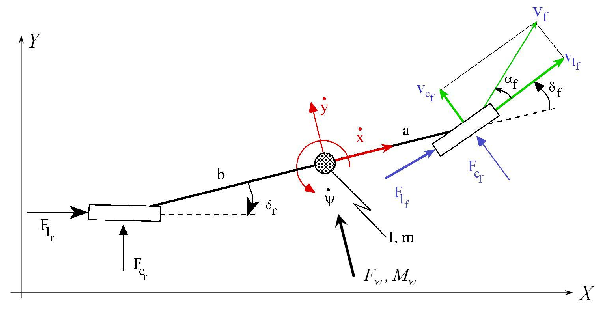
\includegraphics[width=0.80\textwidth,keepaspectratio]{images/01_Vehicle_Dynamical_Model.pdf}
	\caption{The simplified vehicle dynamical model. \cite{Borrelli2005}}
	\label{fig_01:vehicle_dynamical_model}
\end{figure}
Longitudinal and lateral tire forces which are formulated in \ref{Tire_Model} lead to the following forces acting on the center

\begin{subequations} 
	\begin{align} F_y &= F_{l}\sin(\delta) + F_{c}\cos(\delta) \label{eqn:longitudinal_tire_force} \\
	F_x &= F_{l}\cos(\delta) - F_{c}\sin(\delta) 	 \label{eqn:lateral_tire_foce} 
	\end{align} 
\end{subequations}
\par Tire forces, $F_{l} = f_{l}(\alpha, s, \mu, F_z)$, and $F_{c} = f_{c}(\alpha, s, \mu, F_z)$, for each tire are the functions of slip angle ($\alpha$), slip ratio ($s$) road friction coefficient ($\mu$) and normal tire load ($F_{z}$). The slip ratio defined as

\begin{equation}
	\label{eqn:slip_ratio}
	s =
	\begin{cases}
	& \frac{r\omega}{v} - 1 \,\,\text{if}\,\, v > r\omega, \,v \neq 0 \,\, \text{for braking}  \\
	& 1- \frac{r\omega}{v} \,\,\text{if}\,\, v < r\omega, \,\omega \neq 0 \,\, \text{for driving}\\
	\end{cases}   
\end{equation} 
\par The slip angle represents the angle between the wheel velocity and the direction of
the wheel itself:
\begin{equation}
	\label{eqn:slip_angle}
	\alpha = \tan^{-1}\frac{v_{c}}{v_{l}}
\end{equation}
\par In equation \ref{eqn:slip_angle}, $v_{c}$ and $v_{l}$ are the lateral (or cornering) and longitudinal wheel
velocities, respectively, which are expressed as
\begin{subequations} 
	\begin{align} 
	v_l &= v_{y}\sin(\delta) + v_{x}\cos(\delta) \label{eqn:lateral_wheel_velocities} \\
	v_c &= v_{y}\cos(\delta) - v_{x}\sin(\delta) 	 \label{eqn:longitudinal_wheel_velocities}
	\end{align} 
\end{subequations}
and

\begin{subequations} 
	\begin{align} 
	v_{y_{f}} &= \dot{y} + a\dot{\psi} &&v_{y_{r}} = \dot{y} - b\dot{\psi} \label{eqn:lateral_wheel_velocities_I} \\
	v_{x_{f}} &= \dot{x}  &&v_{x_{r}} = \dot{x} \label{eqn:longitudinal_wheel_velocities_II}
	\end{align} 
\end{subequations}
\par $F_{z}$ is distributed between the front and rear wheels based on the geometry of the car model, described by the parameters $a$ and $b$;
\begin{subequations} 
	\label{eqn:normal_tire_load}
	\begin{align} 
	F_{z_{f}} &= \frac{bmg}{2(a+b)} 
	\label{eqn:normal_tire_load_front_wheel} \\
	F_{z_{r}} &= \frac{amg}{2(a+b)} 	 \label{eqn:normal_tire_load_rear_wheel}
	\end{align} 
\end{subequations}
\par Using the equations \ref{eqn:longitudinal_lateral_yaw_second_derivative}-\ref{eqn:normal_tire_load}, the nonlinear vehicle dynamics can be described
 by the following compact differential equation assuming a \textbf{certain slip ratio} ($s$) and \textbf{friction coefficient value} ($\mu$):

\begin{subequations} 
	\label{eqn:nonlinear_system_dynamics}
	\begin{align} 
	\dot{\bm{\xi}} &= f_{s,\mu}(\bm{\xi},u) \\
	\bm{\eta} &= h(\bm{\xi})
	\end{align} 
\end{subequations}
where the state and input vectors are $\bm{\xi}=[y\,\,\dot{y}\,\,x\,\,\dot{x}\,\,{\psi}\,\,\dot{\psi}\,\,Y\,\,X]^{T}$ and $u=\delta_{f}$, respectively, and the output map is given as
\begin{equation}
	\label{eqn:output_eqn}
	{\bm{\eta}} = \begin{bmatrix}
	\psi\\ Y
	\end{bmatrix} = \begin{bmatrix}
	0 & 0 & 0 & 1 & 0 & 0 & 0\\
	0 & 0 & 0 & 0 & 0 & 1 & 0
	\end{bmatrix} \bm{\xi}
\end{equation}

\par Nonlinear kinematic and dynamics equations of 2WS the vehicle can also be represented with control input, $\delta_{f}$, as follows, \cite{Borrelli2005}, \cite{Kong2015}, \cite{Rajamani2011}:
\begin{equation}
	\label{eqn:dynamic_and_kinematic_equations}
	\dot{\bm{\xi}}(t) = \begin{pmatrix}
	\dot{y} \Rightarrow& v\sin(\psi + \beta)\vspace{3mm}\\
	\ddot{y} \Rightarrow& -\dot{x}\dot{\psi} + \frac{2(F_{y_{f}}+F_{y_{r}})}{m} \vspace{3mm} = -\dot{x}\dot{\psi} + \frac{2}{m}(F_{c,f}\cos(\delta_{f})+F_{c,r})\\
	\dot{x} \Rightarrow& v\cos(\psi + \beta)\vspace{3mm}\\
	\ddot{x} \Rightarrow& \dot{y}\dot{\psi} + \frac{2(F_{x_{f}}+F_{x_{r}})}{m} \vspace{3mm}\\
	\dot{\psi} \Rightarrow& r \vspace{3mm}\\
	\ddot{\psi}=\dot{r} \Rightarrow& \frac{1}{I}(\alpha{F}_{y_f}\cos(\delta)-b{F}_{y_r}) \vspace{3mm}\\
	\dot{Y} \Rightarrow& \dot{x}\sin(\psi) + \dot{y}\cos(\psi) \vspace{3mm}\\
	\dot{X} \Rightarrow& \dot{x}\cos(\psi) - \dot{y}\sin(\psi) \vspace{3mm}\\
	\end{pmatrix}  
\end{equation}
where $\beta = \tan^{-1}(\frac{b}{a+b}\tan(\delta_{f}))$ and acceleration of the car is constant, i.e. $\dot{v} = 0$. Forces in $x$- and $y$-directions, $F_x$ and $F_y$, are the function of the forward steering angle, $\delta_{f}$ and longitudinal and lateral tire forces acting on the center. 
\section{Tire Model} \label{Tire_Model}
\par Three possible ways to represent measured tyre data are in use \cite{Bakker1987}:
\begin{itemize}
	\item representation by tables,
	\item representation by graphs,
	\item representation by formula.
\end{itemize}
\par The best way to fulfill the requirements is to find a special function, which through its particular structure is capable of describing the measured data with great accuracy and which has parameters related to the typifying quantities in a simple manner. The formula should, if possible, be able to
describe:
\begin{itemize}
	\item  the side force as a function of slip angle, $\alpha_f\;\& \;\alpha_r$,
	\item  the brake force as a function of longitudinal slip,
	\item the self aligning torque as a function of slip angle.
\end{itemize}
\par The basic form of each of the characteristics of large values the tyre  suggest the use of the sine function as a first step in developing the final formula.
\begin{equation}
\label{eqn:simple_tire_force}
F = D\sin(B\alpha)
\end{equation}
with $F$ standing for either side force, self aligning torque or break force and $\alpha$ denoting slip angle. e. In \ref{eqn:simple_tire_force} $D$ is the peak value and
the product $DB$ equals the slip stiffness at zero
slip. Eq. \ref{eqn:simple_tire_force} does not give a good representation for larger values of $\alpha$. A gradually increasing extension of the X axis appears to be necessary. To accomplish this, the $\arctan$ function has been used. The formula \ref{eqn:simple_tire_force} now changes into:
\begin{figure}[t]
	\centering
	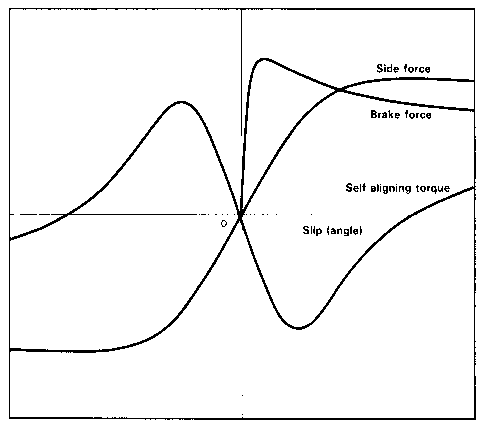
\includegraphics[width=0.75\textwidth,keepaspectratio]{images/Steady-State-Tyre-Characteristics.pdf}
	\caption{Steady-state tyre characteristics.}
	\label{fig_02:steady_state_tyre_characteristics}
\end{figure}
\begin{equation}
\label{eqn:modified_tire_force}
F = D\sin(C\arctan(B\alpha))
\end{equation}
\par In Eq. (2) $D$ is still the peak value, the slip
stiffness at zero slip is now equal to the
$BCD$ (from now on called the stiffness). The
coefficient $C$ governs the shape of the curve in Fig \ref{fig_02:steady_state_tyre_characteristics}.The value of C makes the curve look
like a side force, brake force or a self aligning torque characteristic. With $C$ determined
 by the shape and $D$ determined by the peak value,
only $B$ is left to control the stiffness. Still Eq. \ref{eqn:modified_tire_force} is not good enough to describe
 every possible measured characteristic. There may
 be a need for an additional coefficient which
 makes it possible to accomplish a local extra
 stretch or compression of the curve. The coefficient
 E has been introduced into the formula in such a
way that stiffness and peak value remain
unaffected.
\begin{subequations} 
	\label{eqn:modified_tire_with_force_side_force_char}
	\begin{align} 
	F &= D\sin(C\arctan(B\Phi)) \\
	\Phi &= (1-E)\alpha + \frac{E}{B}\arctan(B\alpha)
	\end{align} 
\end{subequations}
The influence of $E$ on the side force characteristic has been shown in Fig. \ref{fig_03:coefficients-appearing-in-tyre_formula}. Similar effects occur with the self aligning torque and brake force characteristics. The result is an equation with four coefficients, which is able to describe all the measured
characteristics. The four coefficients are:
\begin{figure}[t]
	\centering
	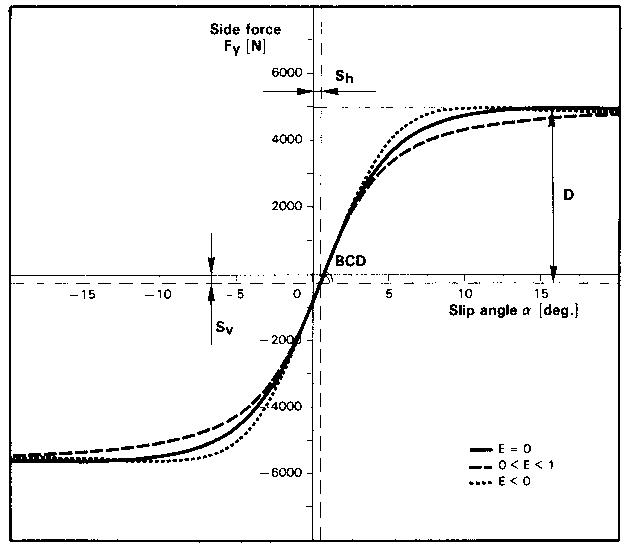
\includegraphics[width=0.75\textwidth,keepaspectratio]{images/Coefficients-Appearing-In-Tyre_Formula.pdf}
	\caption{Coefficients appearing in tyre formula.}
	\label{fig_03:coefficients-appearing-in-tyre_formula}
\end{figure}
\begin{itemize}
	\item $B$ $\Rightarrow$ stiffness factor
	\item $C$ $\Rightarrow$ shape factor
	\item $D$ $\Rightarrow$ peak factor
	\item $E$ $\Rightarrow$ curvature factor
\end{itemize}
\subsection{Influence of Vertical Load}
\par To
reduce the total number of quantified coefficients and to be able to calculate forces and
torques at vertical loads which are different from
the values used in the measurements, it is necessary to include the vertical load explicitly in the
formula. To do so, the coefficients have to be written as a function of the vertical (normal) load, $F_z$. The peak factor, $D$, as a function of $F_z$ may be
approximately represented by the relationship:
\begin{equation}
\label{eqn:tire_model_peak_factor}
D = a_1{F_z}^2 + a_2{F_z}
\end{equation}
\par For the stiffness $BCD$ of the side force characteristic (cornering stiffness), the formula is written as
\begin{equation}
\label{eqn:tire_model_cornering stiffness}
BCD = a_3\sin(a_4\arctan(a_5{F_z}))
\end{equation}
and for the stiffness of both brake force (longitudinal slip stiffness) and self aligning torque (aligning stiffness) characteristics, the approximation is: 
\begin{equation}
\label{eqn:tire_model_longitudinal slip stiffness_aligning stiffness}
BCD = \frac{a_3{F_z}^2 + a_4F_z}{e^{a_5{F_z}}}
\end{equation}
\par The shape factor, $C$, appears to be practically
independent of $F_z$. For above mentioned force types $C$ takes following values: 
\newline \par 
\begin{tabular}{@{$\bullet$ }ll}
	the side force  &: $C = 1.30$ \\
	the brake force &: $C = 1.65$ \\
	the self aligning torque &: $C = 2.40$
\end{tabular}
The stiffness factor $B$ is found by
stiffness by the shape and the peak factor.
\begin{equation}
\label{eqn:tire_model_stiffness_factor}
B = \frac{BCD}{CD}
\end{equation}
\par Finally, the curvature factor $E$ as a function of $F_z$ is given by:
\begin{equation}
\label{eqn:tire_model_curvature_factor}
E = a_6{F_z}^{2} + a_7{F_z} + a_8
\end{equation}
\subsection{Proposed Tyre Formulas}
\subsubsection{Side Force, $F_y$}
\begin{subequations}
	\begin{align}
		\label{eqn:tire_model_side_force}  
		F_y =& D\sin(C\arctan(B\Phi))  + \cancel{\Delta{S_v}} \\
		\Phi =& (1-E)(\alpha+\cancel{\Delta{S_h}})+(E/B)\arctan(B(\alpha+\cancel{\Delta{S_h}})) \\
		D =& a_1{F_z}^2 + a_2{F_z}\\
		C =& 1.30 \\
		B =& \bigg(\frac{a_3\sin(a_4\arctan(a_5F_z)}{CD}\bigg)(1-\cancel{a_{12}|\gamma|})\\
		E =& a_6{F_z}^{2} + a_7{F_z} + a_8 \\
		\Delta{S_h} =& a_9\gamma \\
		\Delta{S_v} =& (a_{10}{F_z}^{2}+ a_{11}F_z)\gamma
	\end{align}
\end{subequations} 
\subsubsection{Self Aligning Torque, $M_z$}
\begin{subequations}
	\begin{align}
	\label{eqn:tire_model_self_aligning_torque}  
	M_z =& D\sin(C\arctan(B\Phi))  + \cancel{\Delta{S_v}} \\
	\Phi =& (1-E)(\alpha+\cancel{\Delta{S_h}})+(E/B)\arctan(B(\alpha+\cancel{\Delta{S_h}})) \\
	D =& a_1{F_z}^2 + a_2{F_z}\\
	C =& 2.40 \\
	B =& \bigg(\frac{a_3{F_z}^2+a_4F_z}{CDe^{a_5{F_z}}}\bigg)(1-\cancel{a_{12}|\gamma|})\\
	E =& (a_6{F_z}^{2} + a_7{F_z} + a_8)/(1-\cancel{a_{13}|\gamma|}) \\
	\Delta{S_h} =& a_9\gamma \\
	\Delta{S_v} =& (a_{10}{F_z}^{2}+ a_{11}F_z)\gamma
	\end{align}
\end{subequations}
\subsubsection{Brake Force, $F_x$}
\begin{subequations}
	\begin{align}
	\label{eqn:tire_brake_force}  
	F_y =& D\sin(C\arctan(B\Phi))  + \cancel{\Delta{S_v}} \\
	\Phi =& (1-E)\alpha+(E/B)\arctan(B\alpha) \\
	D =& a_1{F_z}^2 + a_2{F_z}\\
	C =& 1.65 \\
	B =& \frac{a_3{F_z}^{2} + a_4{F_z}}{CDe^{a_5{F_z}}}\\
	E =& a_6{F_z}^{2} + a_7{F_z} + a_8 \\
	\Delta{S_h} =& a_9\gamma \\
	\Delta{S_v} =& (a_{10}{F_z}^{2}+ a_{11}F_z)\gamma
	\end{align}
\end{subequations} 
\subsection{Matlab Code for Longitudinal and Lateral Tire Forces}
\lstinputlisting{tire_model.m}
\begin{figure}[h]
	\centering
	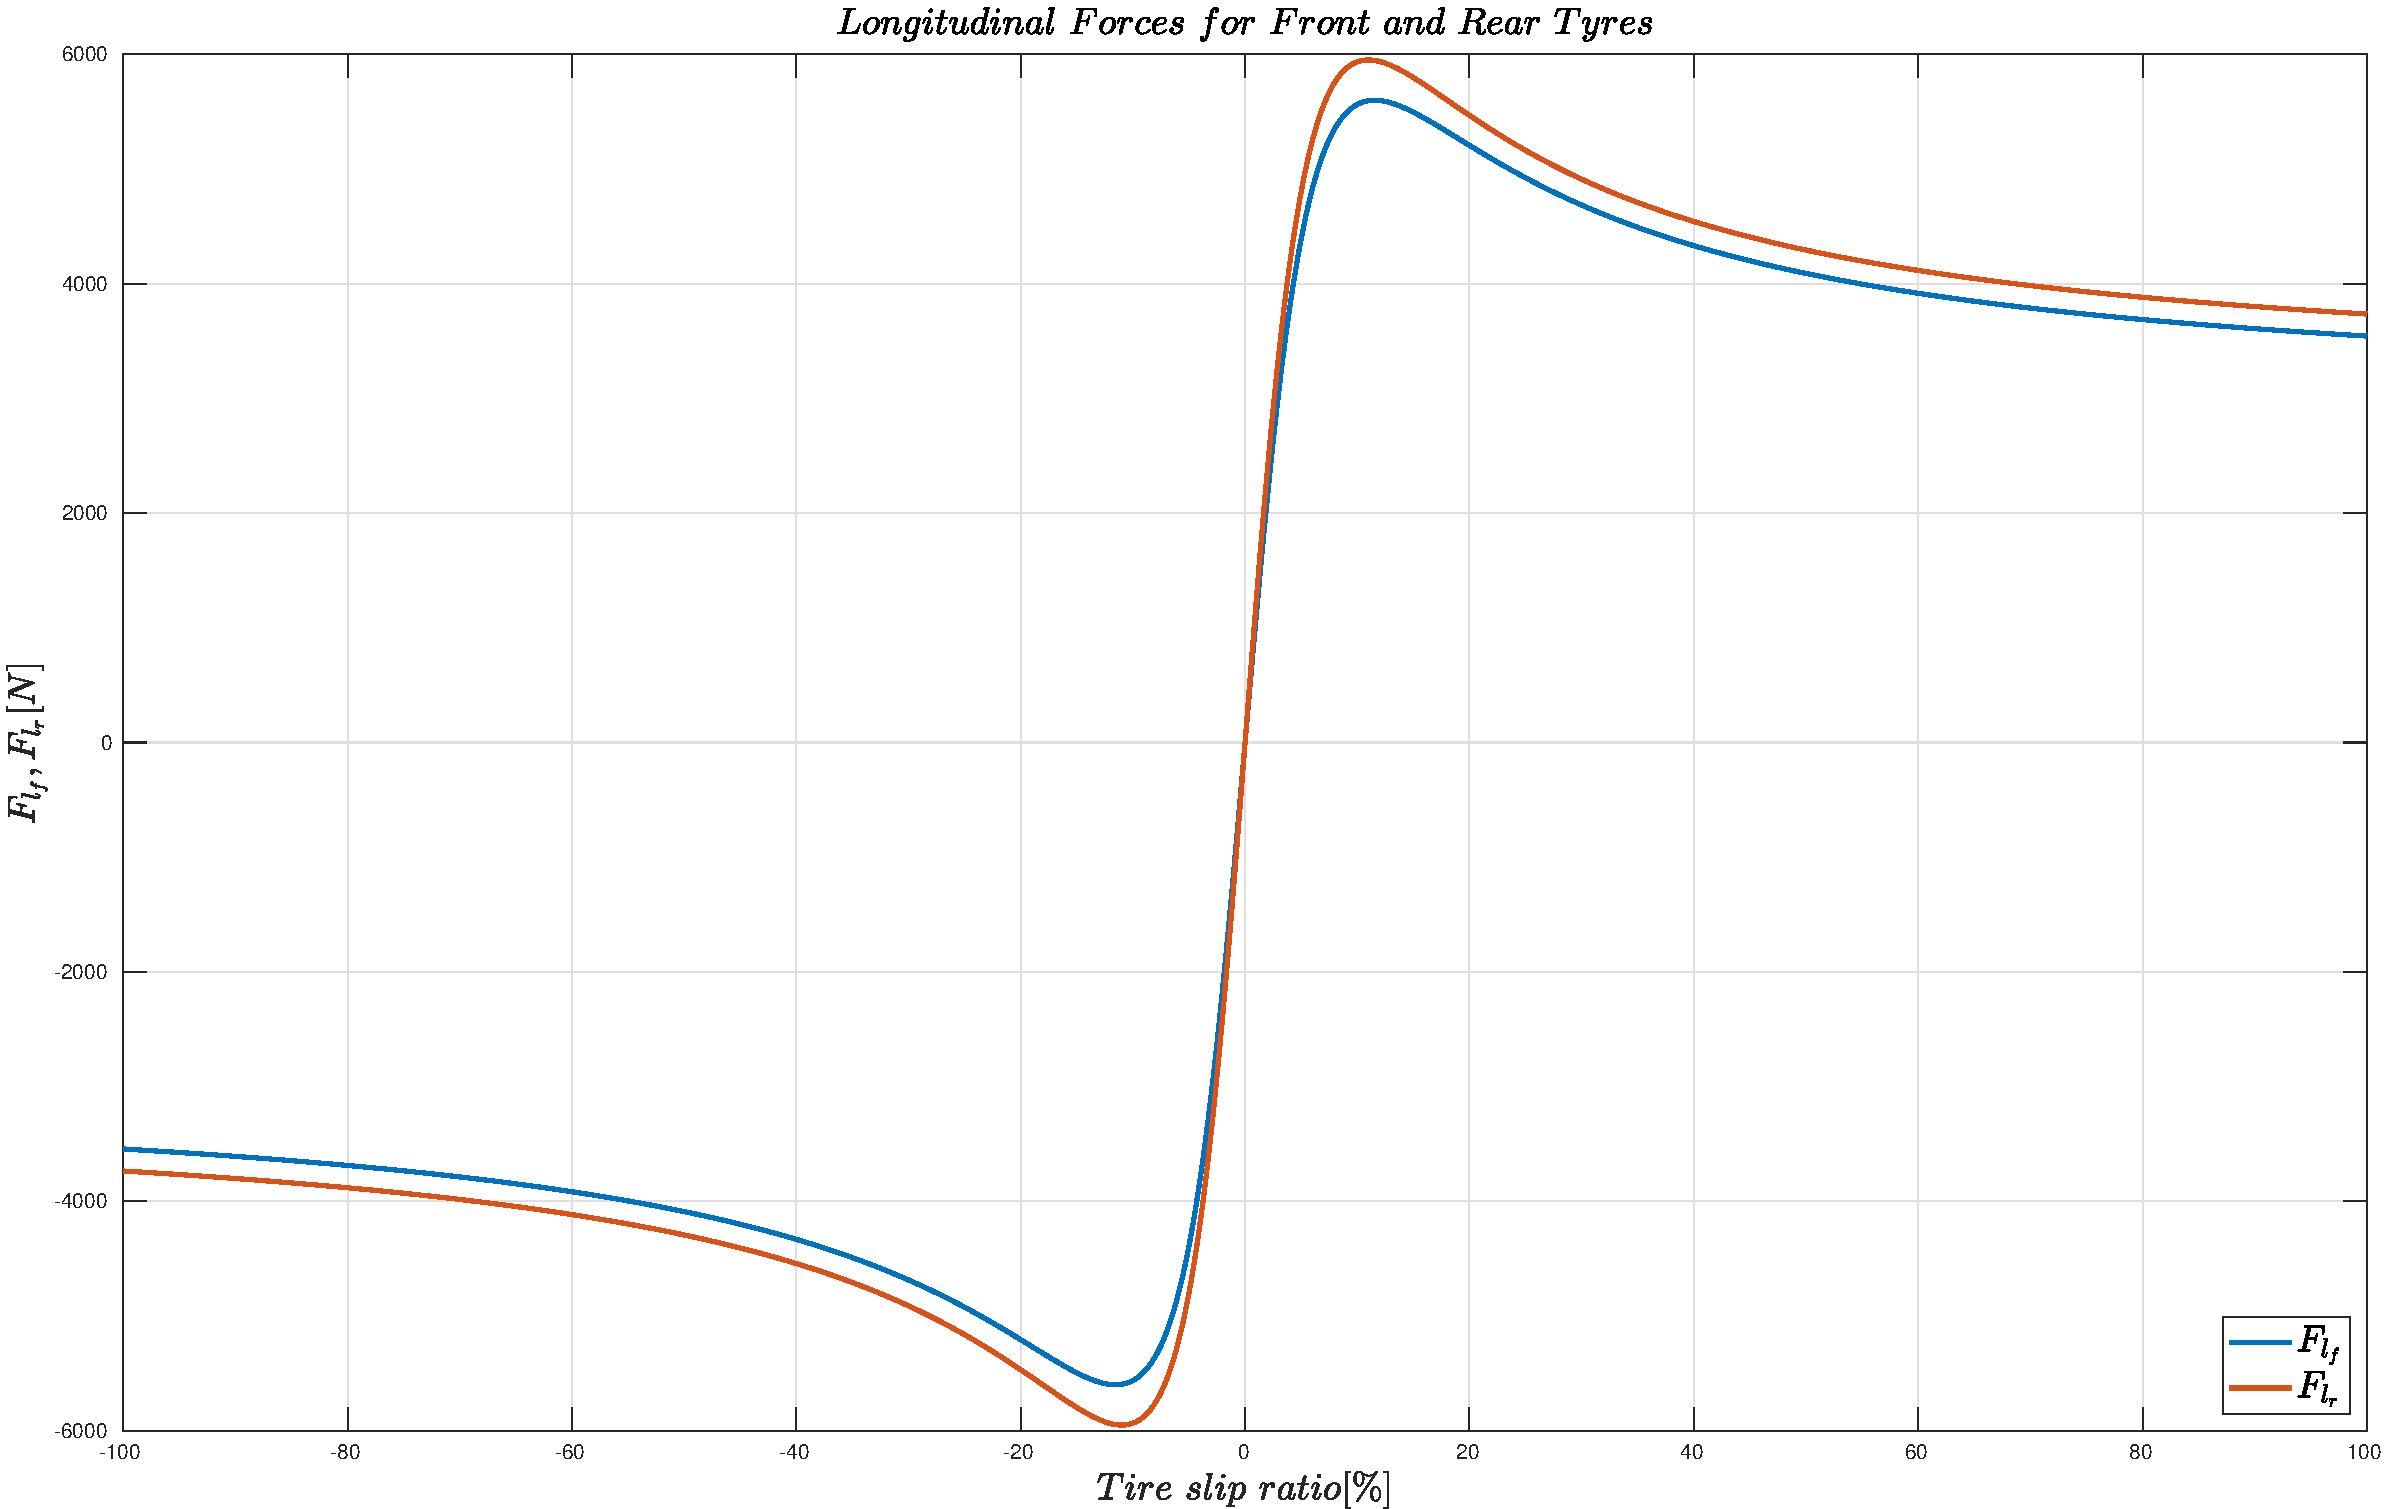
\includegraphics[width=0.95\textwidth,keepaspectratio]{images/Longitudinal-Forces.pdf}
	\caption{Longitudinal forces of front and rear tyres.}
	\label{fig_04:longitudional_forces}
\end{figure}

\textbf{\begin{figure}[h]
	\centering
	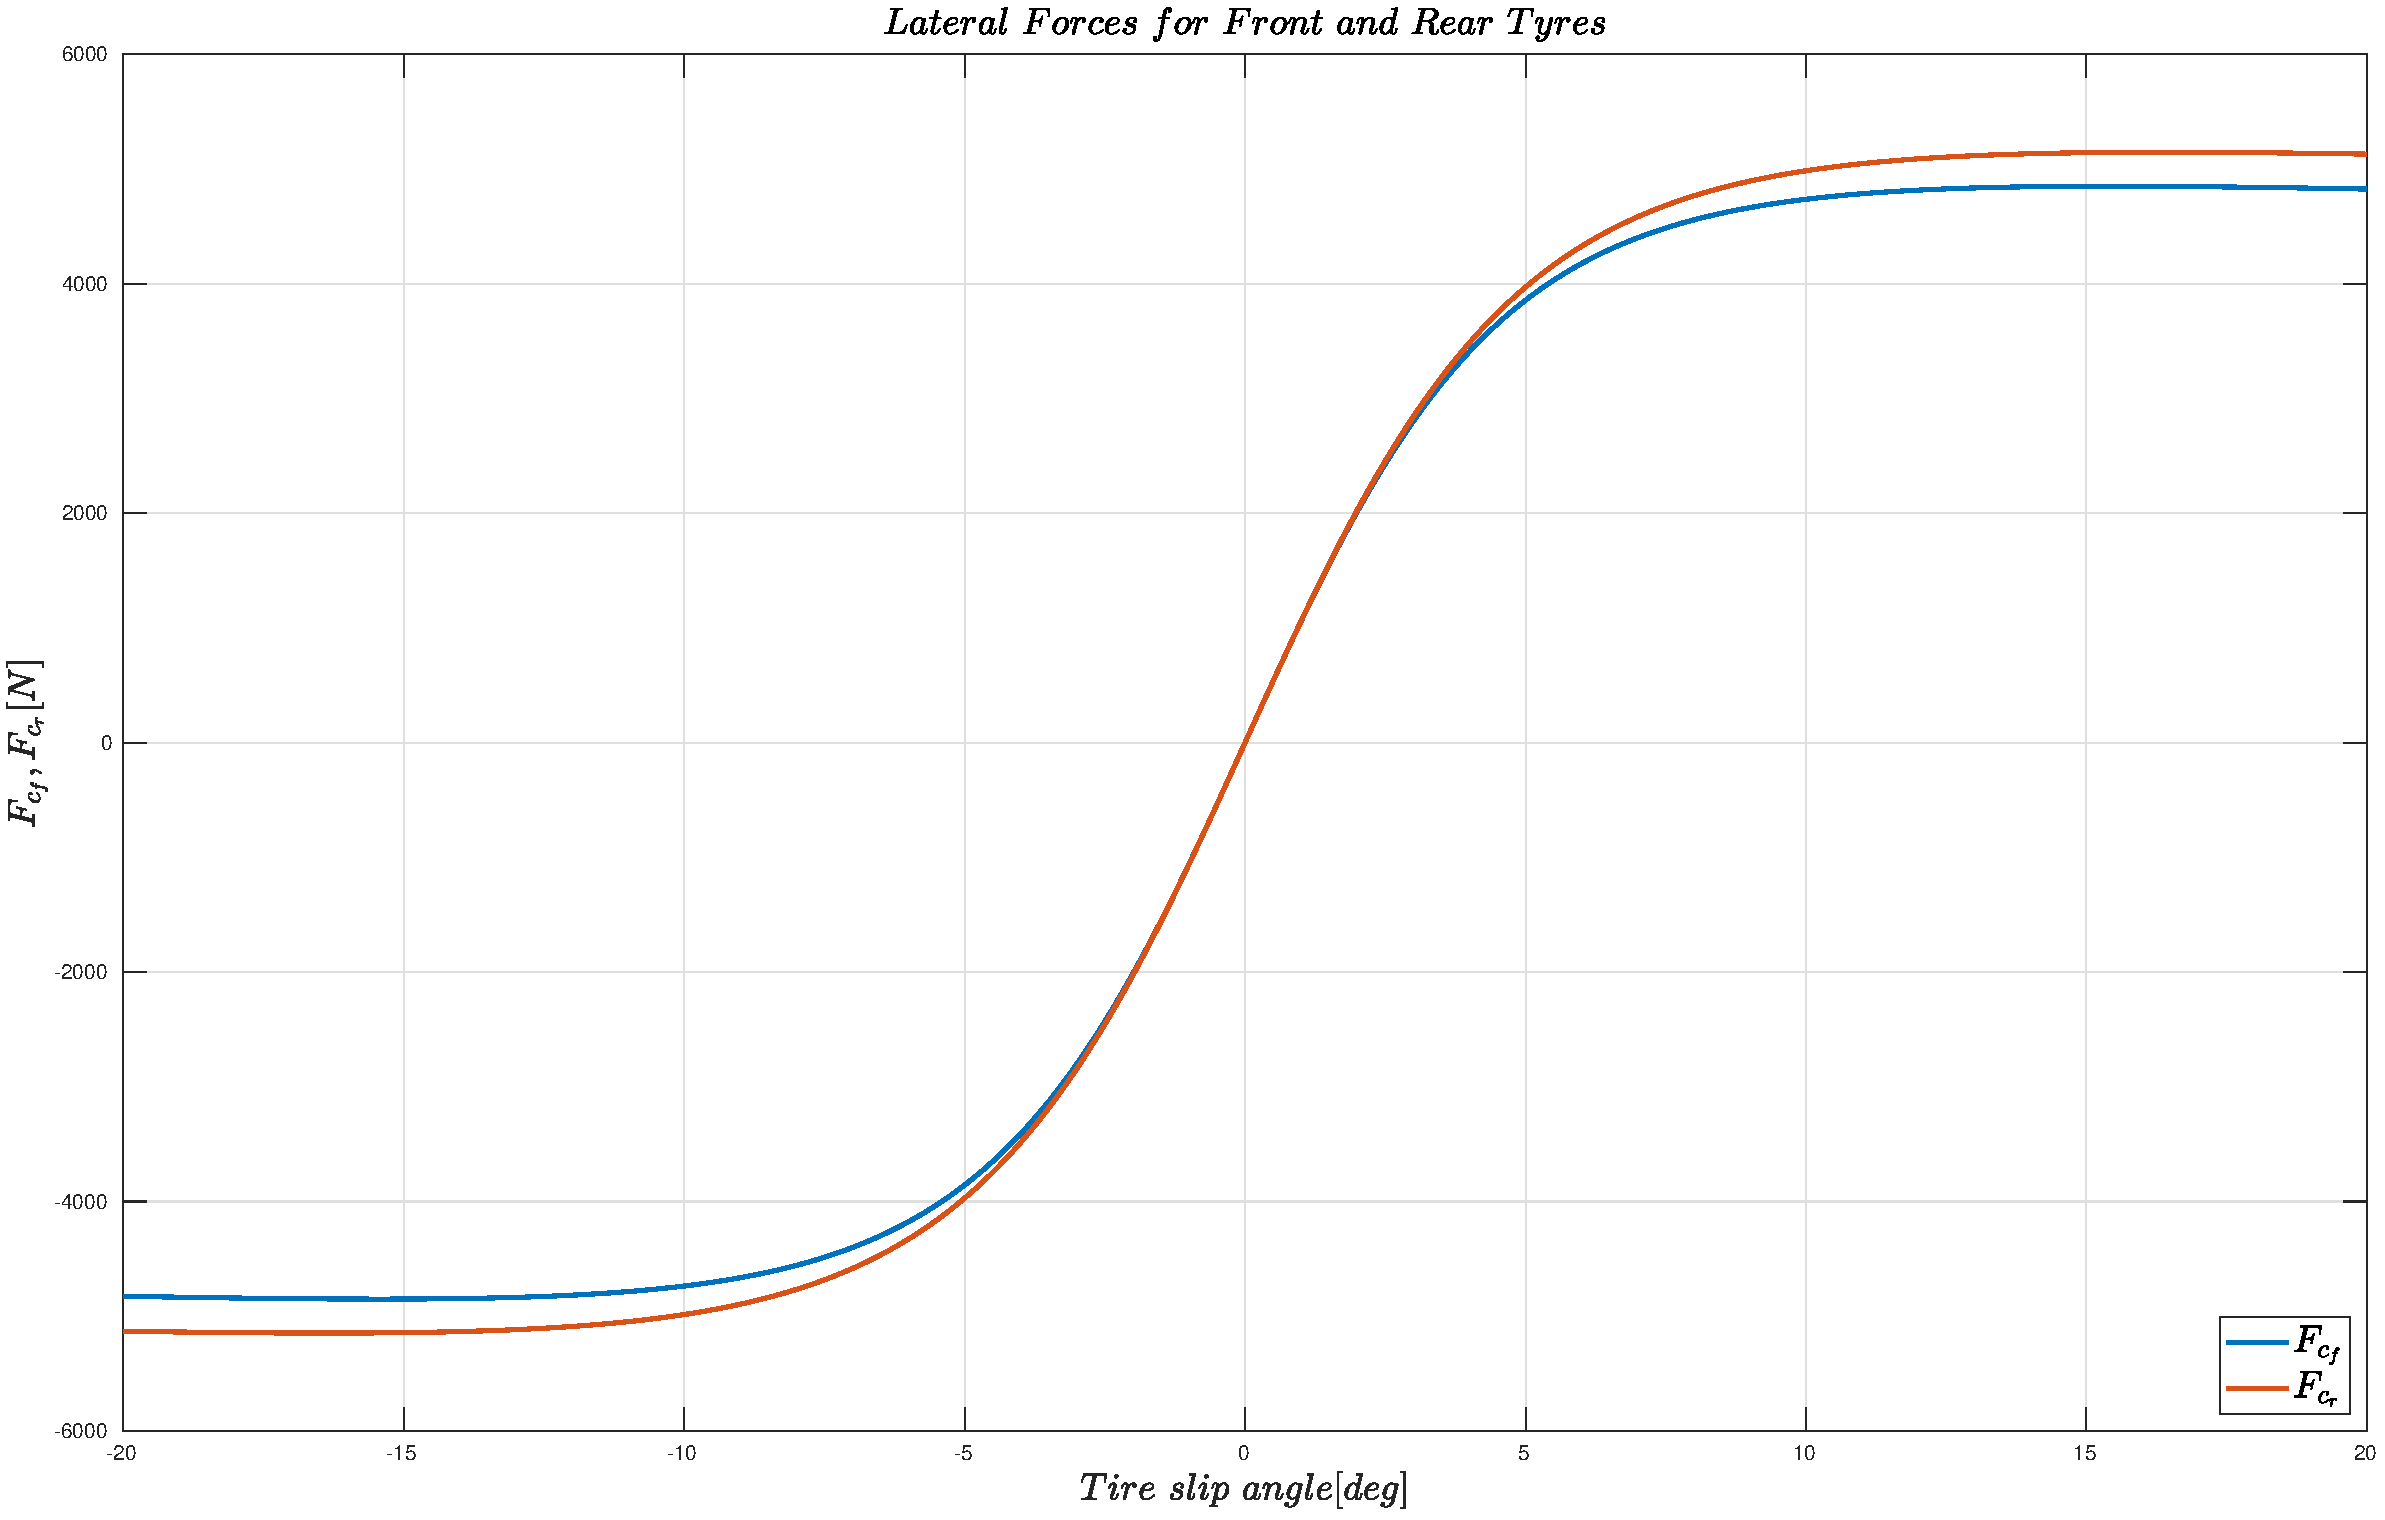
\includegraphics[width=0.95\textwidth,keepaspectratio]{images/Lateral-Forces.pdf}
	\caption{Lateral forces of front and rear tyres.}
	\label{fig_05:lateral_forces}
\end{figure}}

\section{Problem Formulation}
A finite dimensional optimal control problem can be obtained by discretizing the system dynamics as indicated in \ref{eqn:nonlinear_system_dynamics} with the Euler method,
\begin{subequations} 
	\label{eqn:discretize_system}
	\begin{align} 
	{\bm{\xi}}(k+1) &= f^{dt}_{s,\mu}(\bm{\xi}(k),u(k)) \\
	\bm{\eta}(k) &= h(\bm{\xi}(k))
	\end{align} 
\end{subequations}
where the $\Delta u$ formulation is used, i.e., $u(k) = u(k-1)+\Delta u(k)$ and $u(k)=\delta_{f}(k)$, $\Delta u(k)=\Delta\delta_{f}(k)$. Objective or the cost function of the system can be defined as follows:
\begin{align}
\label{eqn:Optimization_Cost_Function}  
\bm{\textit{J}}(\bm{\xi}(k),\Delta\bm{U}_{t})  =& \sum\limits_{i=1}^{H_{p}}(\hat{\bm{\eta}}_{t+i,t}-{\bm{\eta}}_{{ref}_{t+i,t}})^{T}\,\bm{\bm{Q}}\,(\hat{\bm{\eta}}_{t+i,t}-{\bm{\eta}}_{{ref}_{t+i,t}})  \nonumber\\ +&\sum\limits_{i=0}^{H_{c}-1}\Delta{u}_{t+i,t}\,{R}\,\Delta{u}_{t+i,t}\, \\
=& \sum\limits_{i=1}^{H_{p}} \norm[\Big]{\hat{\bm{\eta}}_{t+i,t}-{\bm{\eta}}_{{ref}_{t+i,t}}}^{2}_{\bm{Q}} + \sum\limits_{i=0}^{H_{c}-1}  \norm[\Big]{\Delta{u}_{t+i,t}}^{2}_{R} \nonumber
\end{align} 
In \ref{eqn:Optimization_Cost_Function} the first summand reflects the desired performance on target tracking, the second summand is a measure of the steering effort. At each time step t the following finite horizon optimal control problem is solved:
\begin{equation} 
	\label{eqn:mpc_problem_formulation}
	\begin{aligned}
	& \underset{\bm{\Delta{U}}}{\text{min}}
	& & \bm{\textit{J}}(\bm{\xi}(k),\Delta\bm{U}_{t})  \\
	& \text{st.}
	& & {\bm{\xi}}(k+1) = f^{dt}_{s,\mu}(\bm{\xi}(k),u(k)),\,\,\, k = t,\dots,t+H_{p} \\
	& 
	& & \bm{\eta}(k) = h(\bm{\xi}(k)),\,\,\, k = t,\dots,t+H_{p} \\
	& 
	& & \delta_{f,min} \leq u_{k,t} \leq \Delta\delta_{f,max} \,\,\, k = t,\dots,t+H_{c}-1 \\
	& 
	& & \Delta\delta_{f,min} \leq \Delta u_{k,t} \leq \Delta\delta_{f,max} \,\,\, k = t,\dots,t+H_{c}-1 \\
	& 
	& & u_{k,t} = u_{k,t-1} + \Delta u_{k,t}
	\end{aligned} 
\end{equation}
When the above optimization problem is solved at time $t$ for the current observed states $\bm{\xi}_{t,t}$, sequence of the optimal control inputs, $\Delta\bm{U}^{*}_{t}=[\Delta u^{*}_{t,t},\dots,\Delta u^{*}_{t+H_{c}-1,t}]^{T}$, within the specified control horizon. The resulting state feedback control law is,
\begin{equation}
	\label{eqn:control_law}
	\delta_{f}(t) = \delta_{f}(t-1) + \Delta{u}^{*}_{t,t}
\end{equation} 

\section{Double Lane Change on Snow Using Active Steering}
\subsection{Scenario Description}
The reference signals (desired tracking signals) $\mu_{ref} = \begin{bmatrix} \psi_{ref}\\ Y_{ref} \end{bmatrix}$ are specified by the following set of equations: 
\begin{subequations} 
	\label{eqn:reference_path_angle_equations}
	\begin{align} 
	{Y}_{ref}&= \frac{d_{y_1}}{2}(1 + \tanh(z_1))-\frac{d_{y_2}}{2}(1 + \tanh(z_2)) \\
	{\psi}_{ref} & = \arctan\Bigg(d_{y_1}\Big(\frac{1}{\cosh(z_1)}\Big)^2\Big(\frac{1.2}{d_{x_1}}\Big) - d_{y_2}\Big(\frac{1}{\cosh(z_2)}\Big)^2\Big(\frac{1.2}{d_{x_2}}\Big) \Bigg)  \\
	z_1 &= \frac{shape}{d_{x_1}}(X-X_{s_1})-\frac{shape}{2} \\
	z_2 &= \frac{shape}{d_{x_2}}(X-X_{s_2})-\frac{shape}{2}
	\end{align} 
\end{subequations}
where $shape=2.4$, $d_{x_1} = 25$, $d_{x_2} = 21.95$, $d_{y_1} = 4.05$, $d_{y_2} = 5.7$, $X_{s_1} = 27.19$ and
$X_{s_2} = 56.46$. Unless differently specified, the following parameters have been used for the 2WS NLMPC controller.

\subsection{Matlab Code for Checking Reference Generator}

\begin{figure}[h]
	\centering
	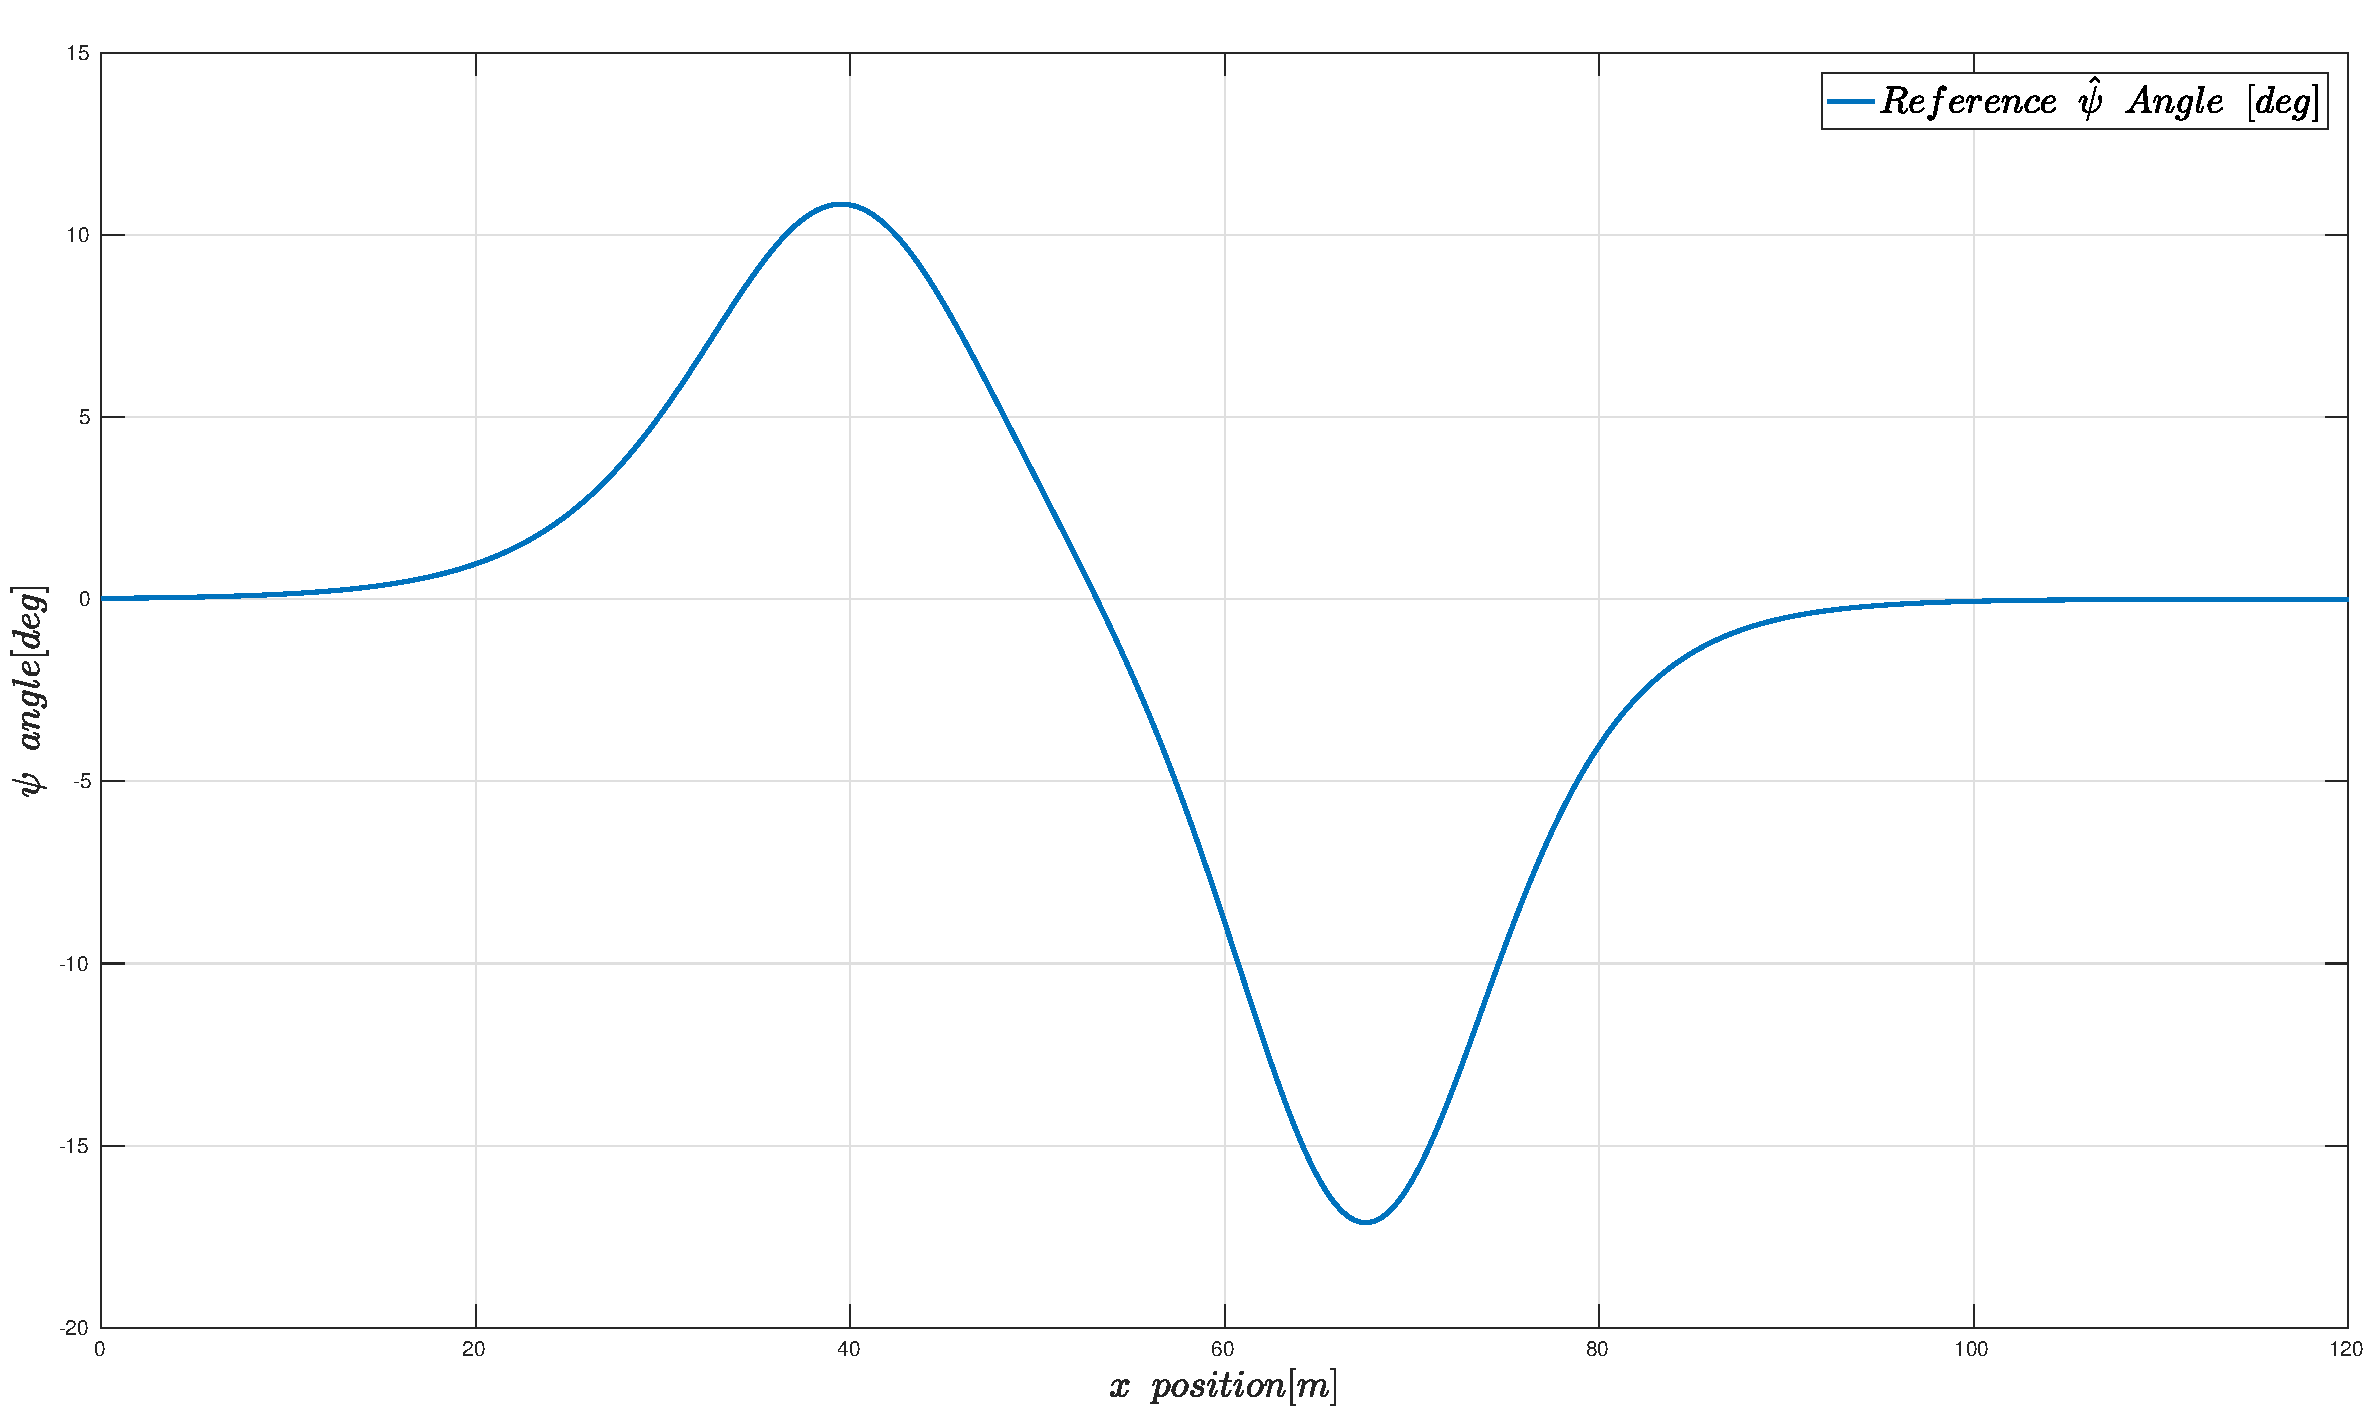
\includegraphics[width=0.95\textwidth,keepaspectratio]{images/Reference-Yaw-Angle.pdf}
	\caption{Reference $\psi$ angle in degree.}
	\label{fig_04:reference_yaw_angle}
\end{figure}

\begin{figure}[t]
	\centering
	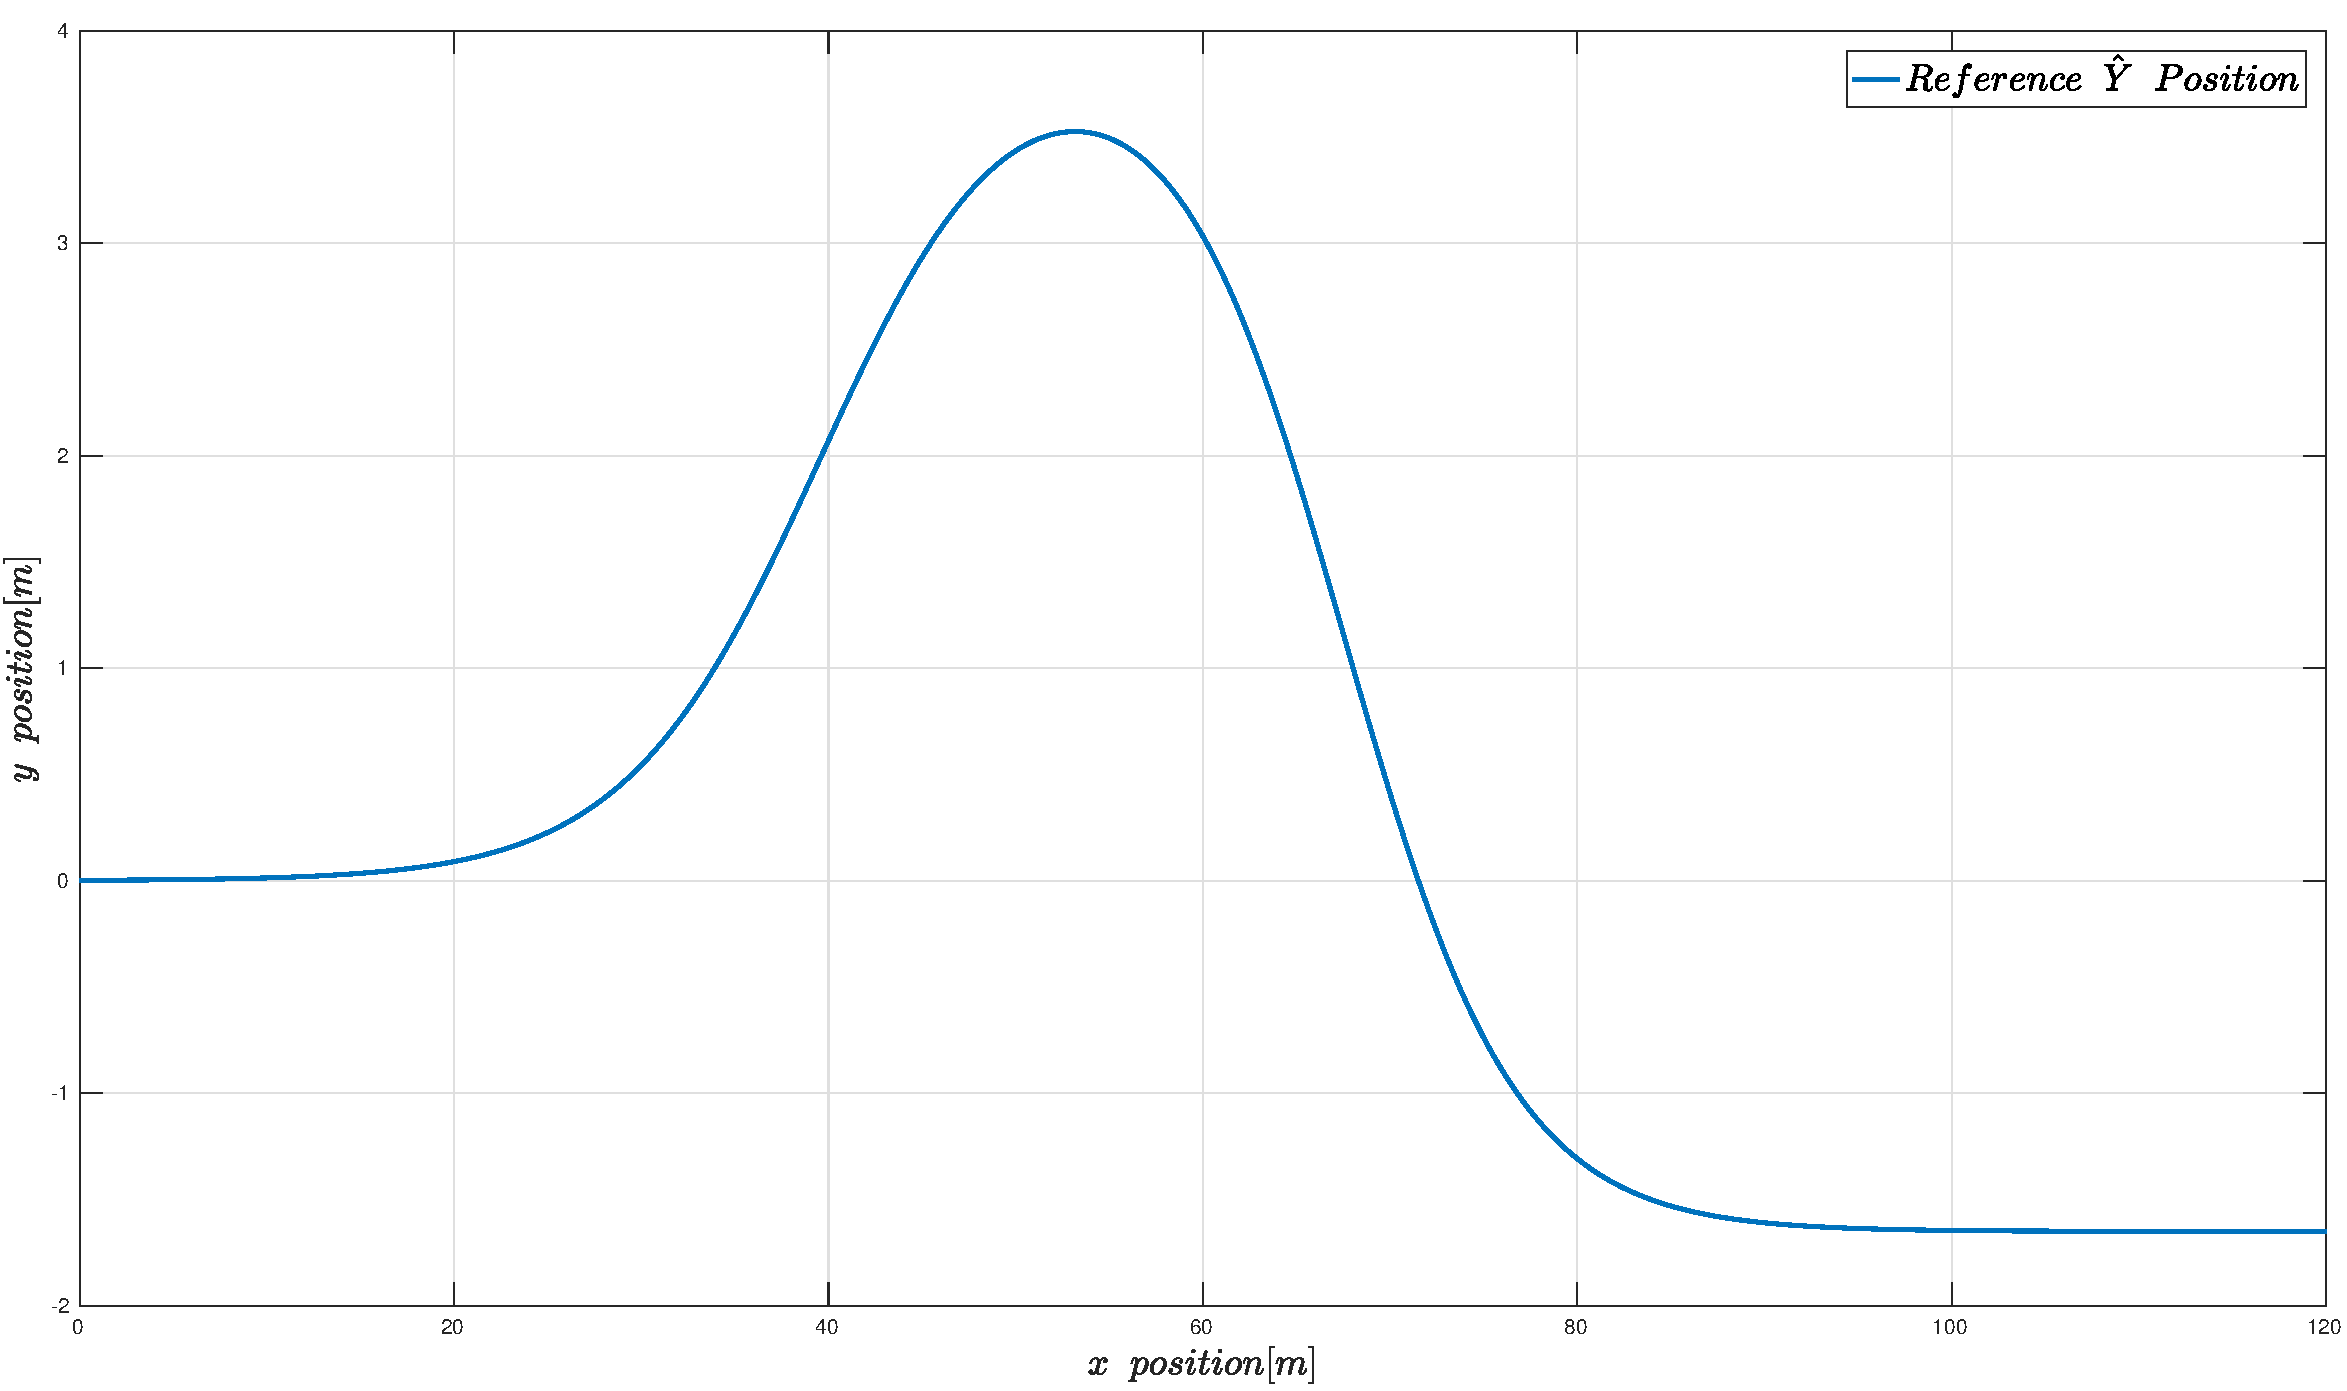
\includegraphics[width=0.95\textwidth,keepaspectratio]{images/Reference-Y-Position.pdf}
	\caption{Reference $\psi$ angle in degree.}
	\label{fig_05:reference_Y_position}
\end{figure}

\lstinputlisting{path_generator.m}

\begin{itemize}
	\item sample time: $T = 0.05$ sec;
	\item constraints on maximum and minimum steering angles $\ang{-30}$ $\leq$ $\delta_{f}$ $\leq$
$\ang{30}$
	\item constraints on maximum and minimum changes in steering angles $\ang{-20}$/s $\leq$ $\Delta\delta_{f}$ $\leq$ $\ang{20}$/s
\end{itemize}
The controller tuning parameters at a given longitudinal vehicle speed are the prediction horizon $H_p$, control horizon $H_c$ and the weighting matrices $Q$ and $R$.
\section{Simulation Results}
\subsection{Simulation Results via MATLAB \& YALMIP}
\textbf{Dependencies For YALMIP}
\begin{enumerate}
	\item Find a suitable folder for yalmip installation and create a folder, go to the folder in MATLAB command window

	e.g. /home/cagdas/Documents/OptimizationTools/yalmip/YALMIP-master (on Linux) be sure you have permission to access,
	\item Download YALMIP from website:
\url{https://yalmip.github.io/download/}

	and copy this .zip file to the folder above
	\item Copy and past the following 3 lines matlab command window
	\\ $>>$ unzip('YALMIP-master.zip','yalmip')
	\\ $>>$ addpath(genpath([pwd filesep 'yalmip']));
	\\ $>>$ savepath
	\item Test YALMIP: run the following command in MATLAB command window, check available optimization tools among lists
	\\ $>>$ yalmiptest
\end{enumerate}

\begin{figure}[!ht]
	\centering
	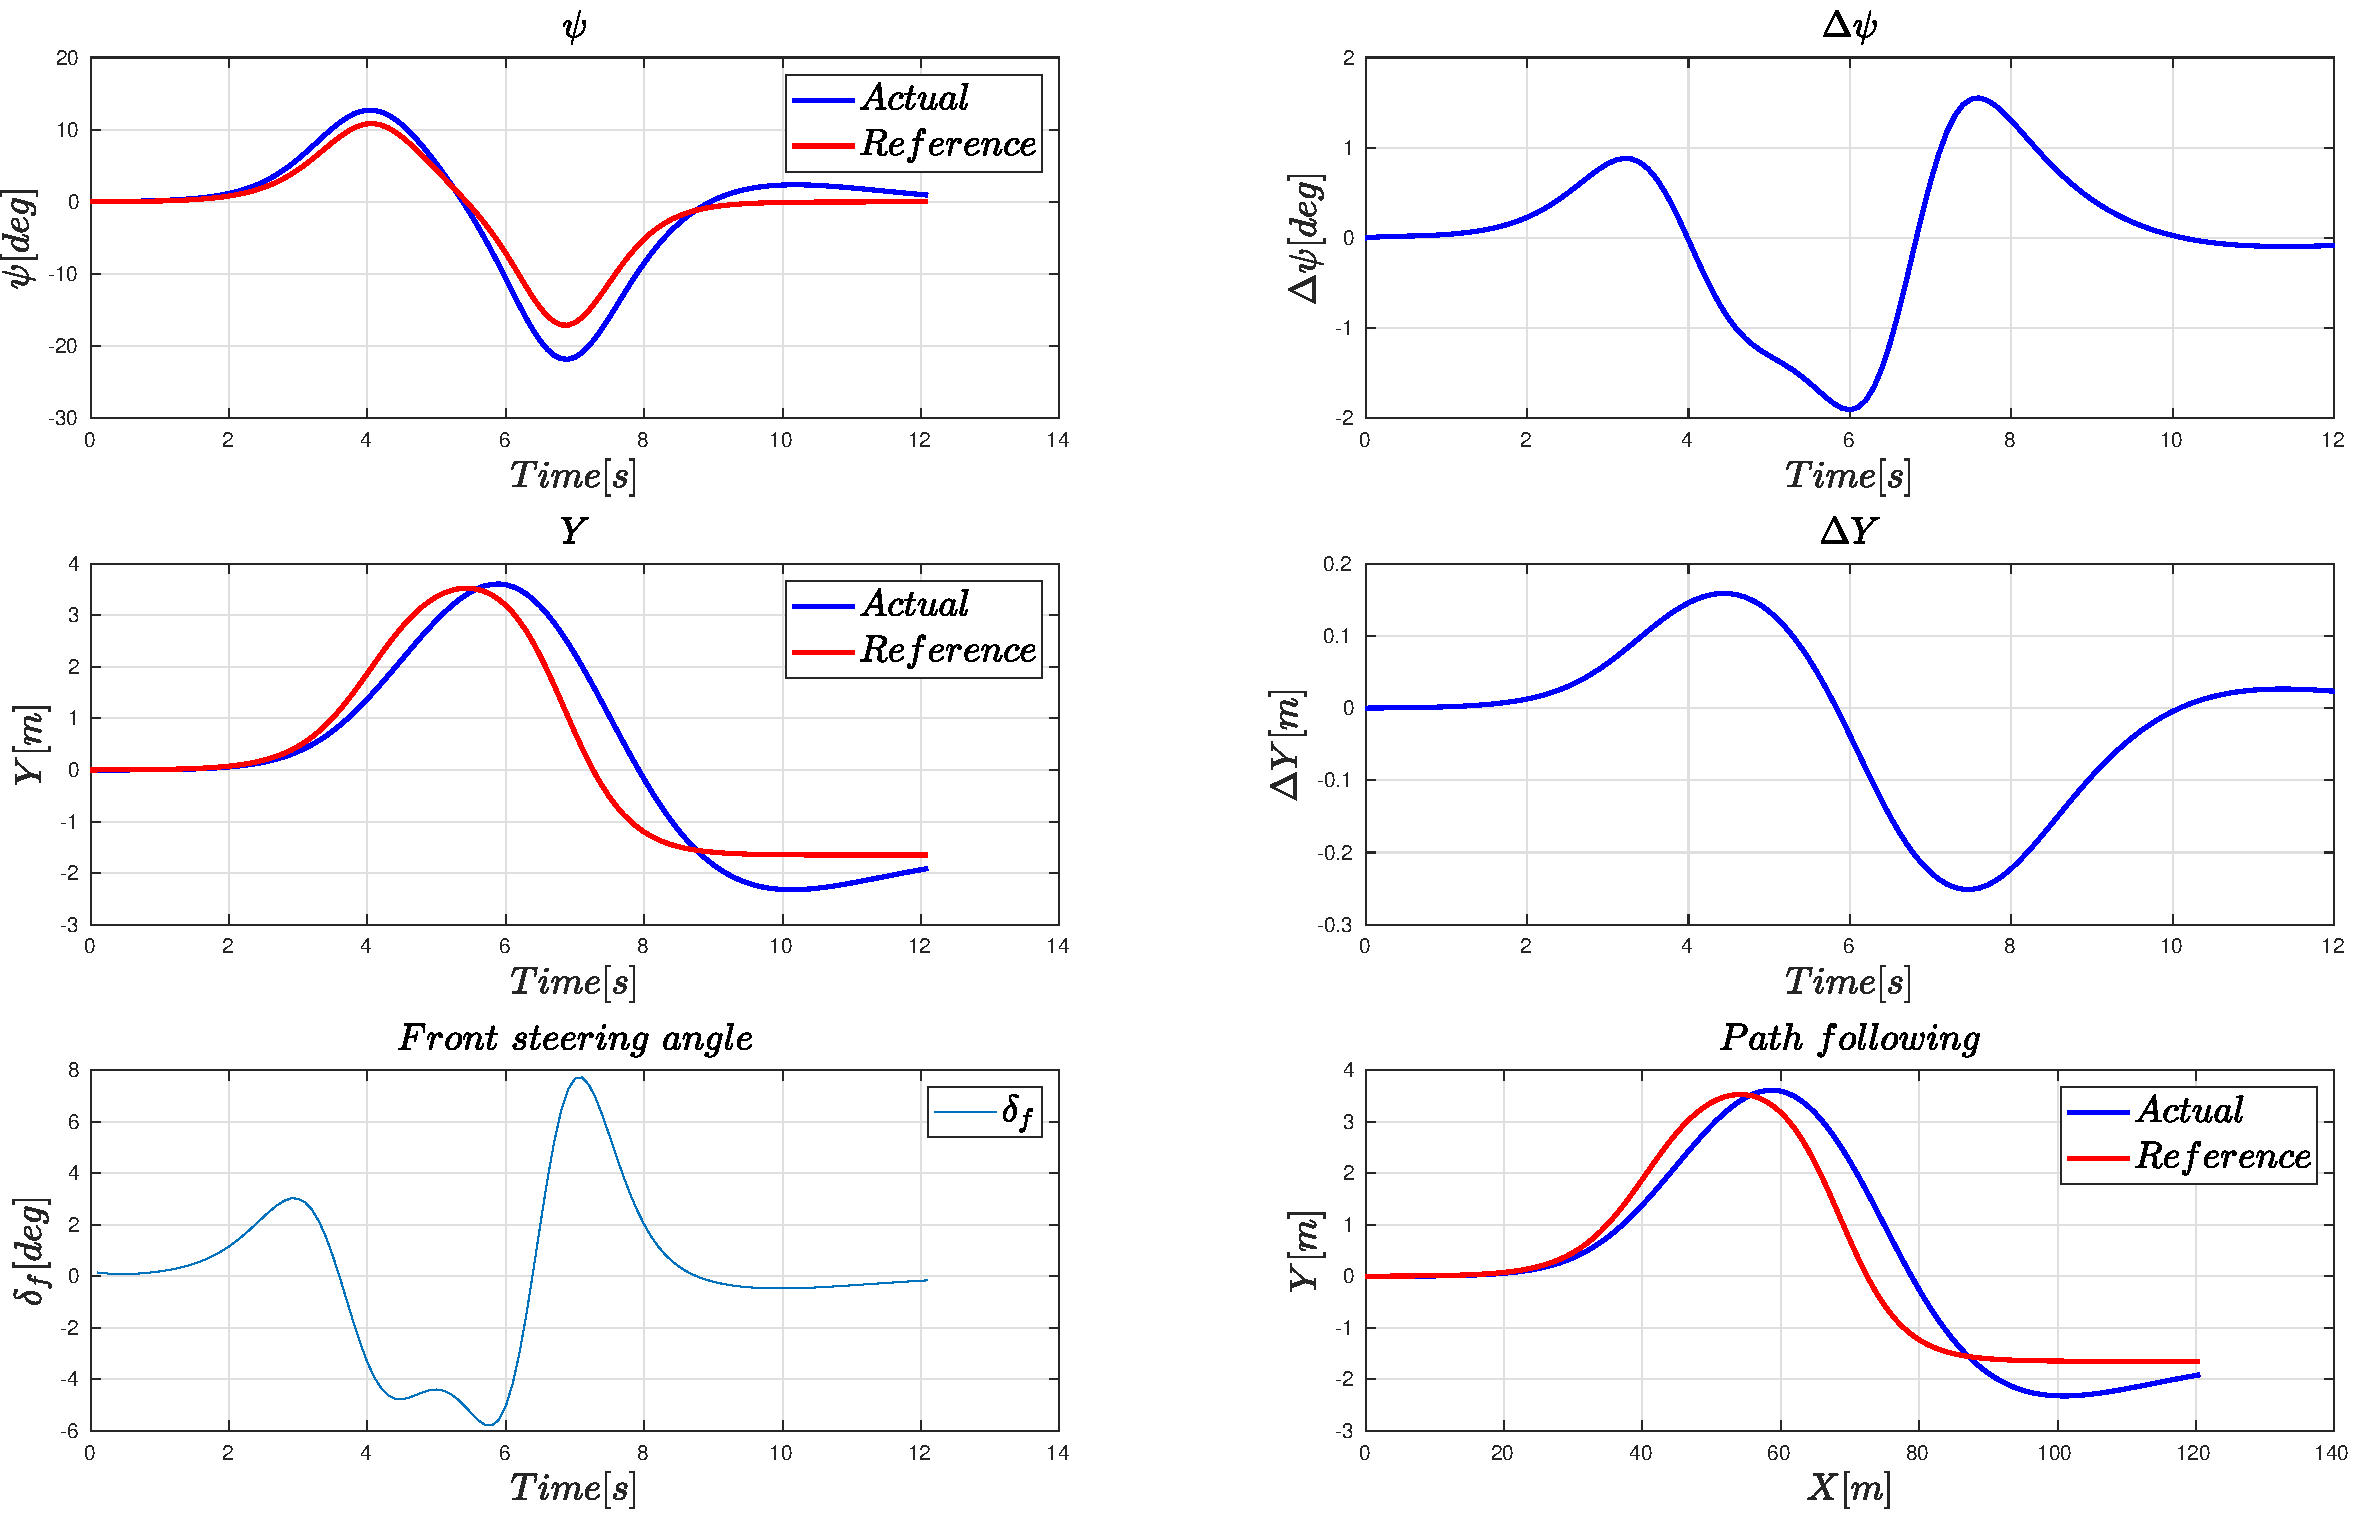
\includegraphics[width=0.95\textwidth,keepaspectratio]{images/Double_Lane_Change_Maneuver_MATLAB_01.pdf}
	\caption{(MATLAB) Double lane change maneuver at $10$ m/s with $H_p$ $=$ $7$ and $H_c$ $=$ $7$}
	\label{fig_08:double_lane_change_maneuver_01}
\end{figure}

\begin{figure}[!hb]
	\centering
	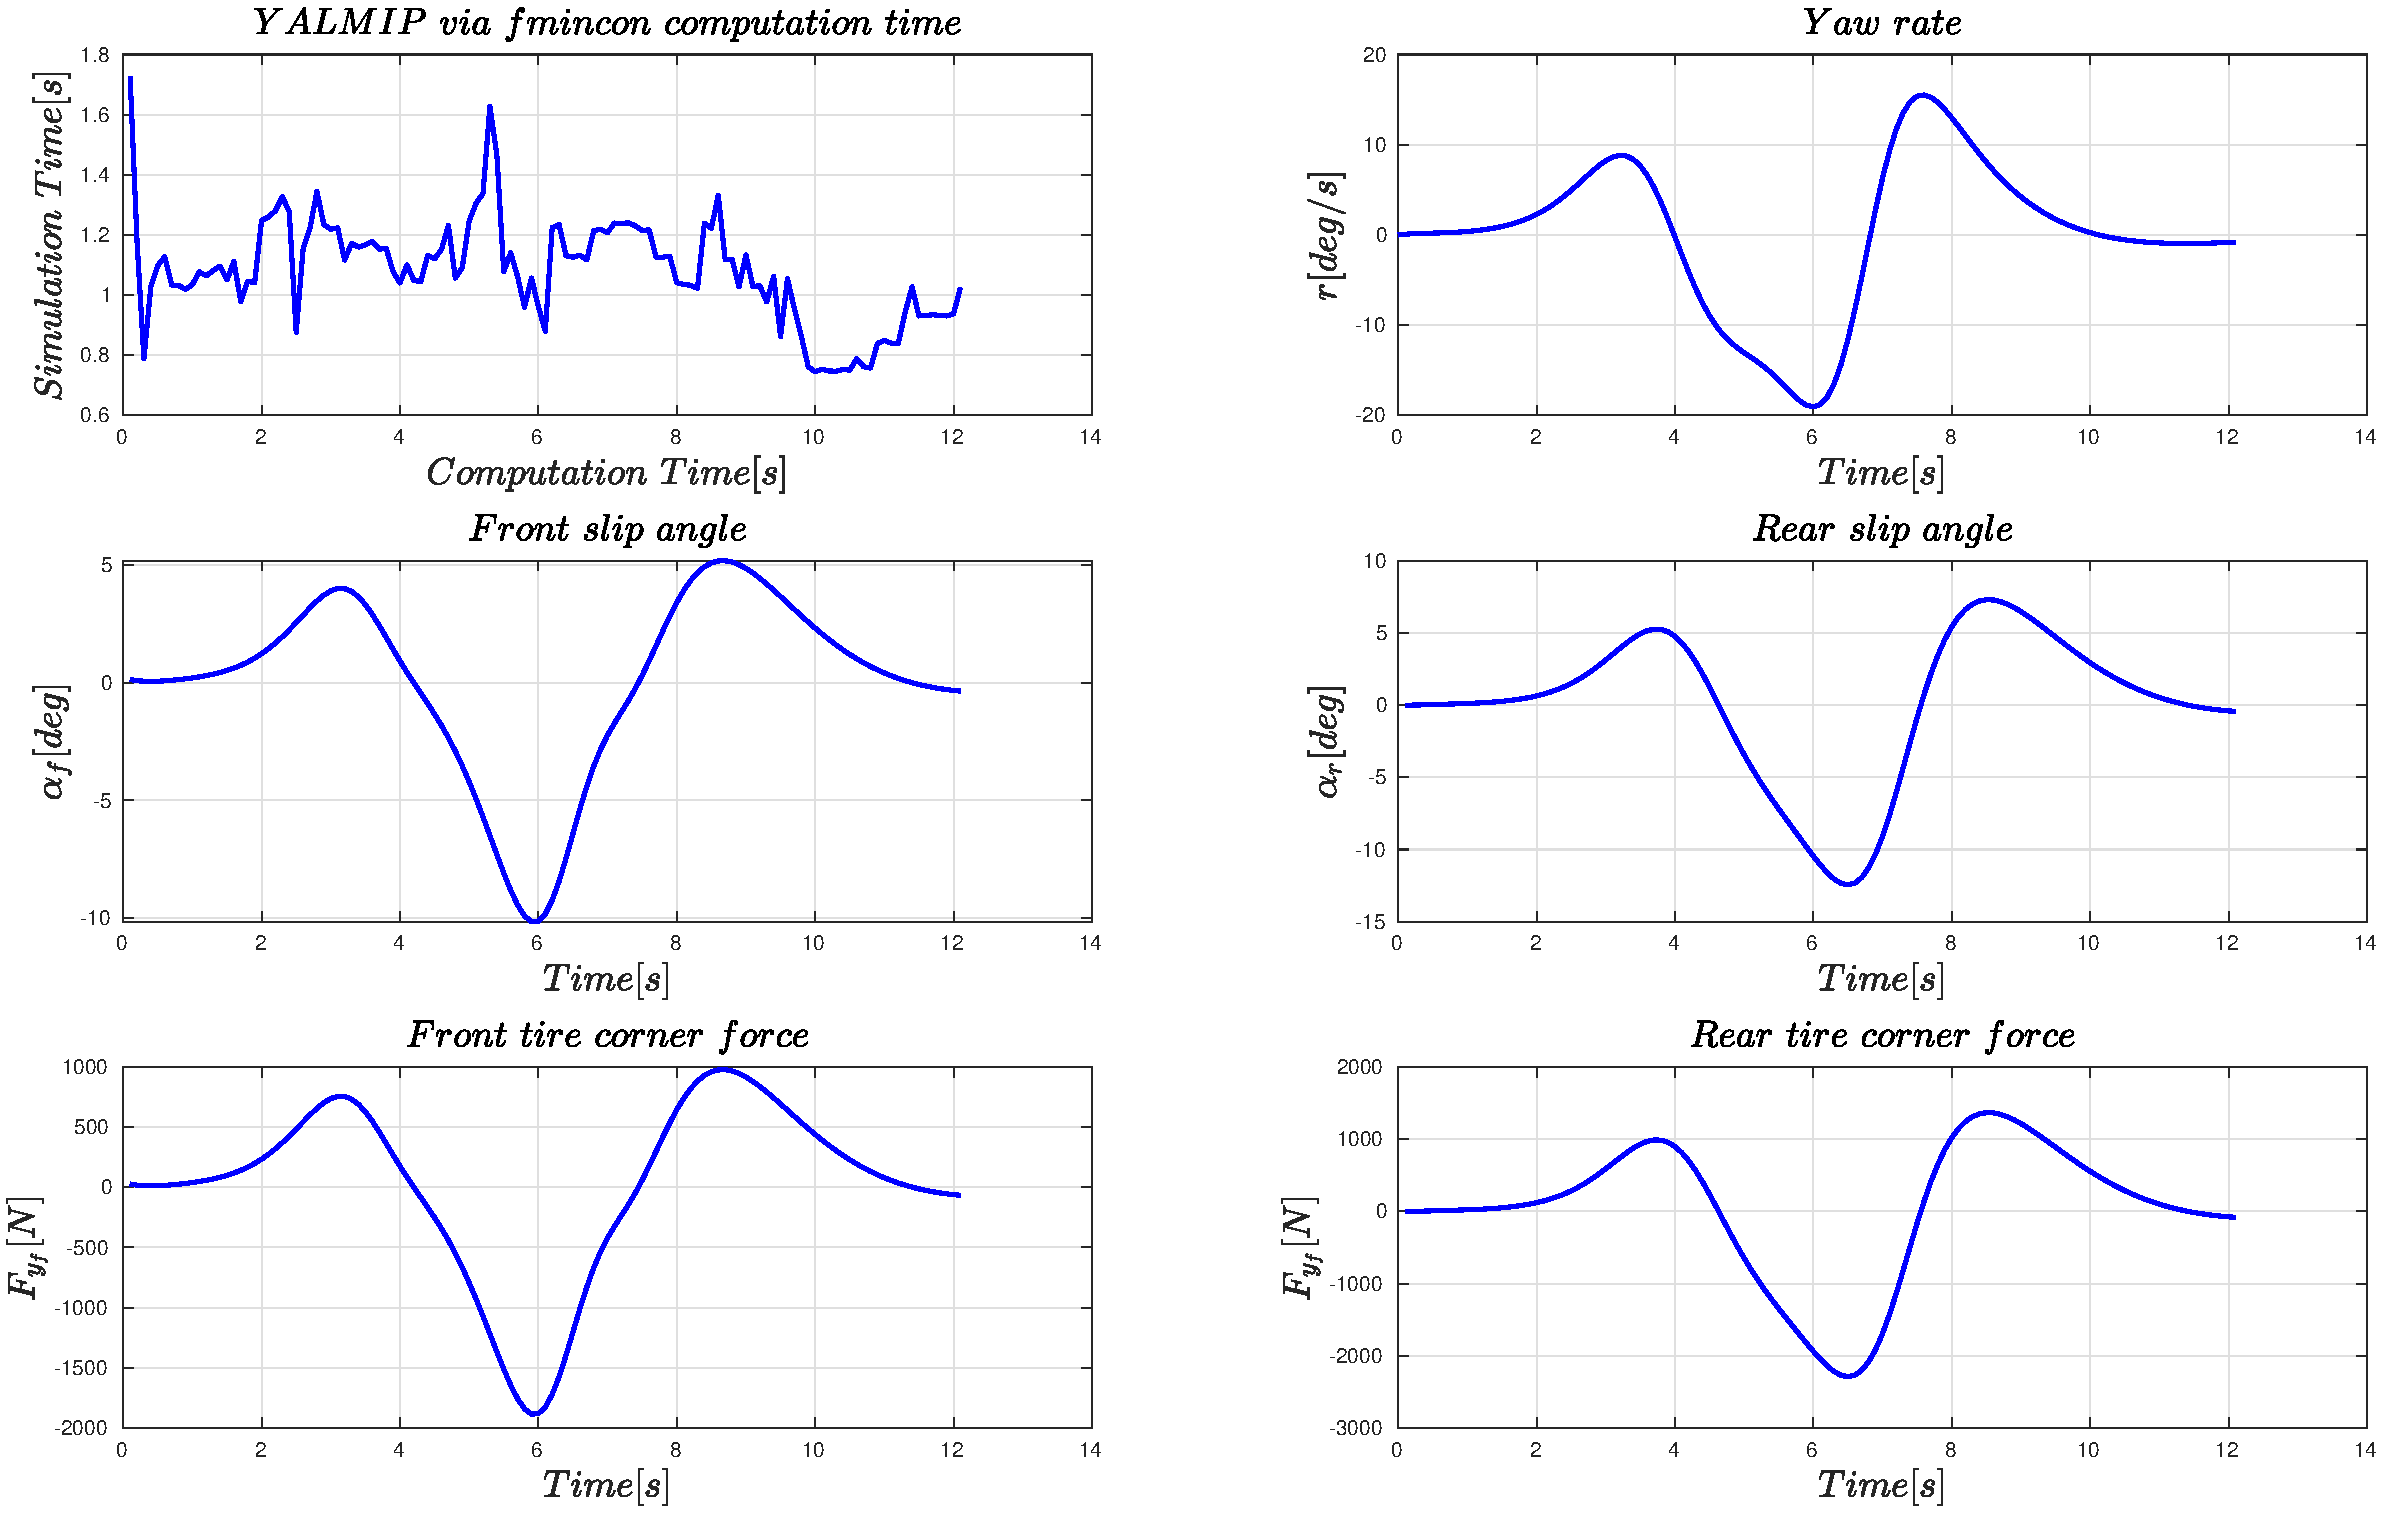
\includegraphics[width=0.95\textwidth,keepaspectratio]{images/Double_Lane_Change_Maneuver_MATLAB_02.pdf}
	\caption{(MATLAB) Double lane change maneuver at $10$ m/s with $H_p$ $=$ $7$ and $H_c$ $=$ $7$. YALMIP computation time, yaw rate, tire forces and slip angles.}
	\label{fig_09:double_lane_change_maneuver_02}
\end{figure}

\subsection{Simulation Results via c++ (IPOPT, cppAD, matplotlibcpp)}
\textbf{Dependencies For C++ Implementation}
\begin{enumerate}
	\item cmake $>=$ 3.5
	\item gcc/g++ $>=$ 5.4
	\item Ipopt and CppAD: Please refer to \href{https://github.com/udacity/CarND-MPC-Project/blob/master/install_Ipopt_CppAD.md}{this document} for installation instructions.
	\item \href{http://eigen.tuxfamily.org/index.php?title=Main_Page}{Eigen} This is already part of the source codes.
\end{enumerate}
\textbf{Basic Build Instructions}
\begin{enumerate}
	\item Make a build directory: \textbf{mkdir build \&\& cd build}
	\item Compile: \textbf{cmake .. \&\& make}
	\item Run it: \textbf{./active\_steering\_mpc}
\end{enumerate}
\begin{figure}[!ht]
	\centering
	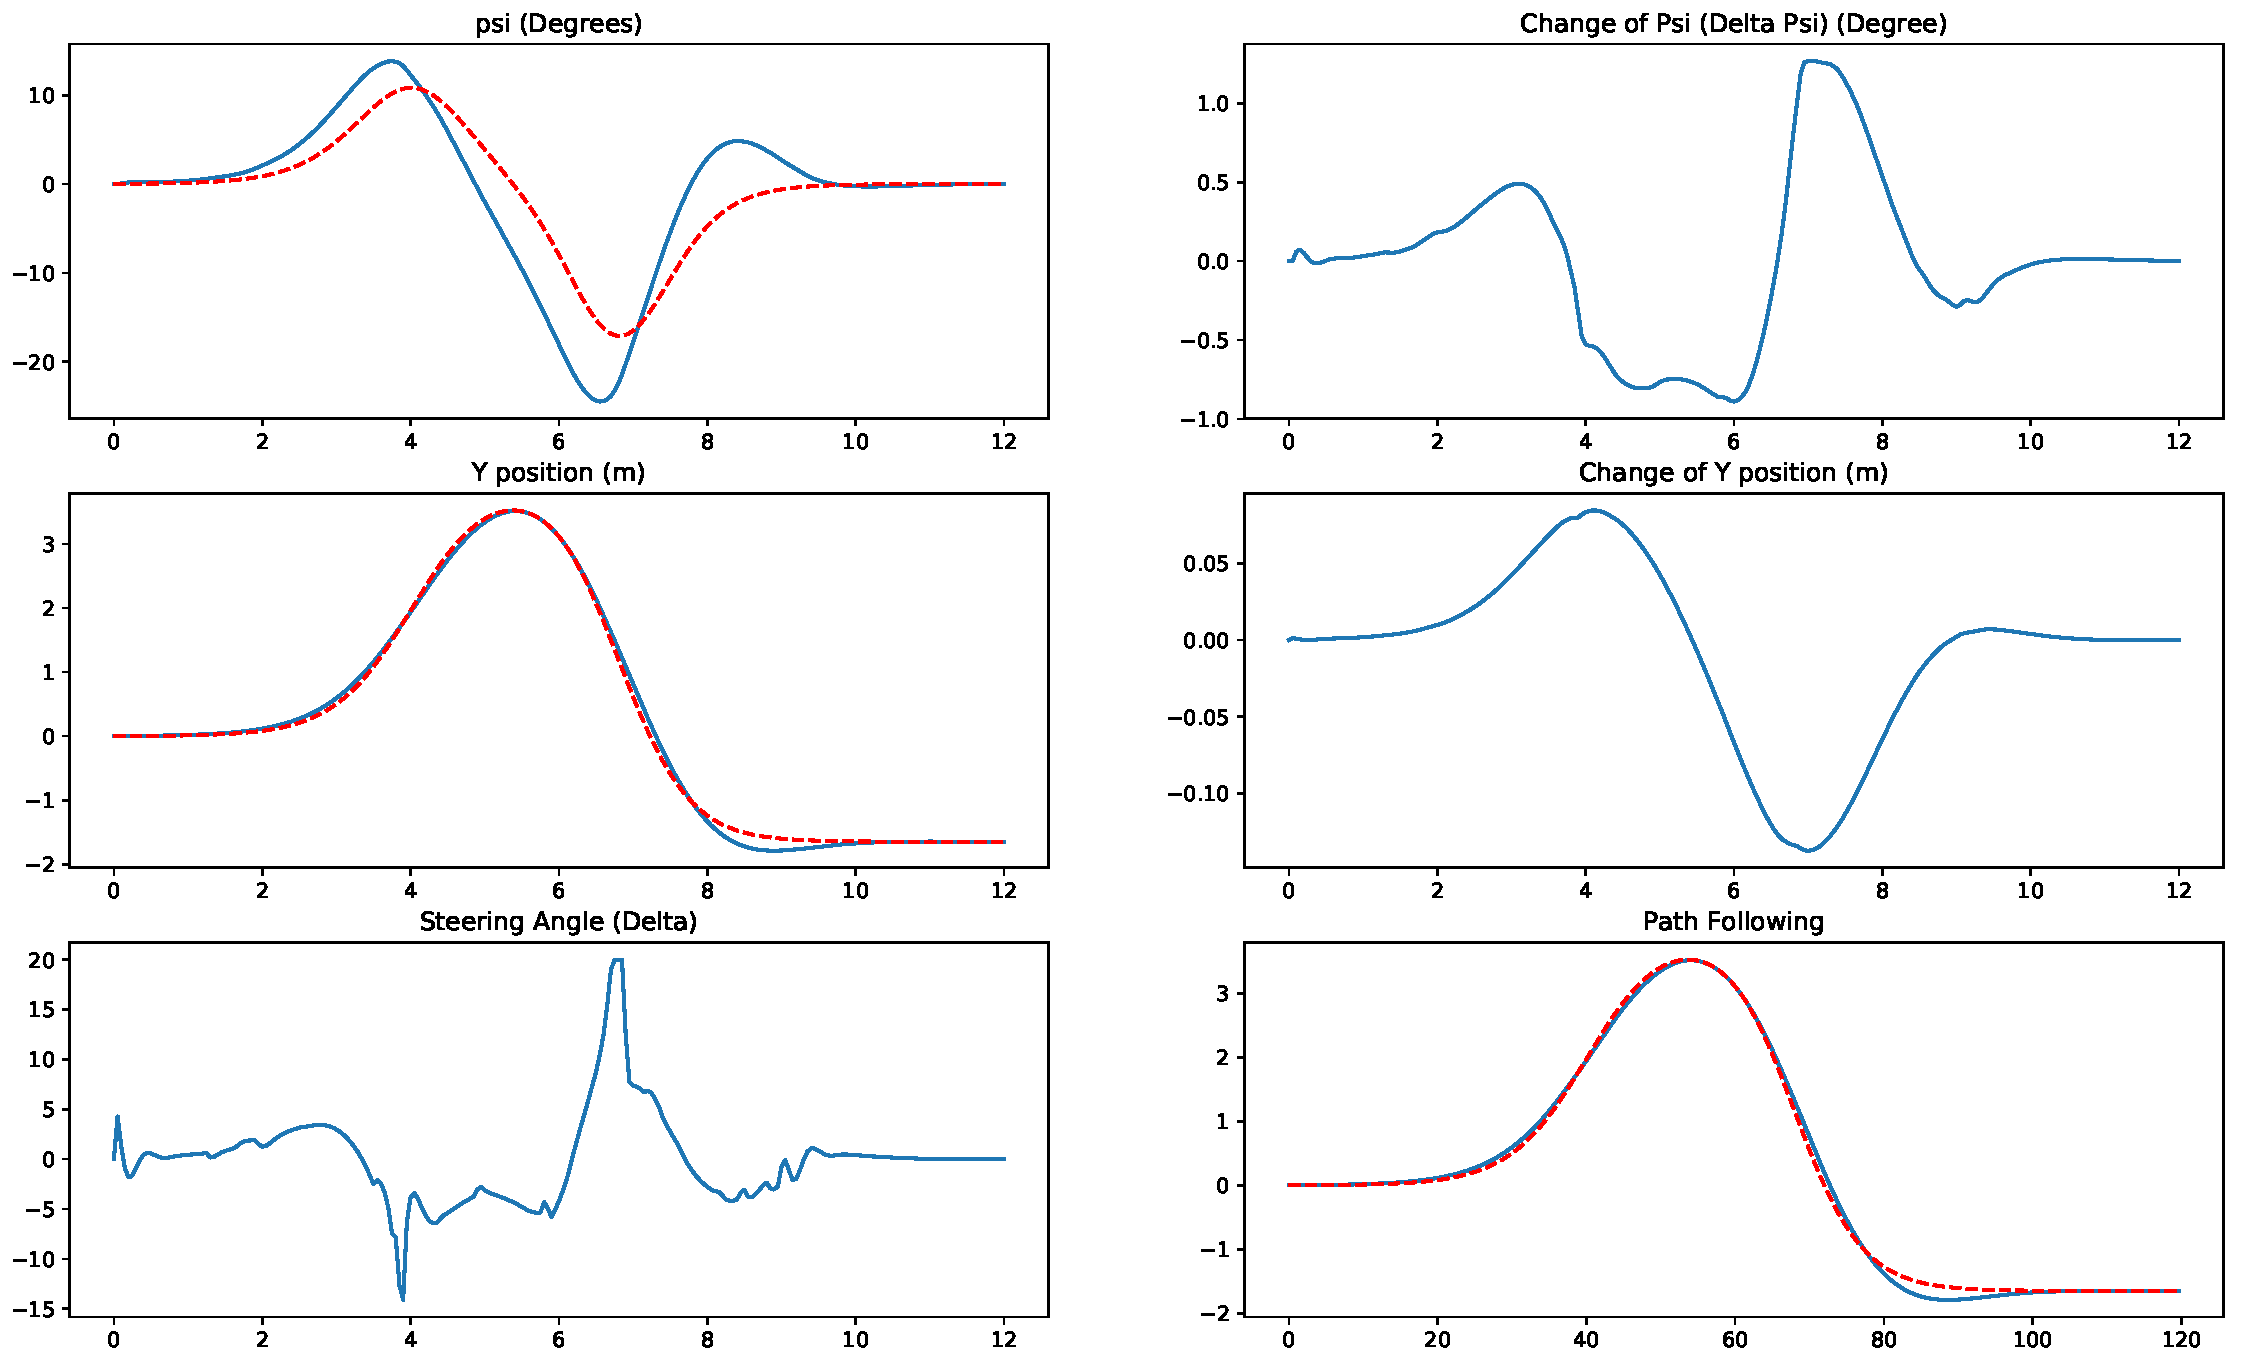
\includegraphics[width=0.95\textwidth,keepaspectratio]{images/Double_Lane_Change_Maneuver_cpp_01.pdf}
	\caption{(c++) Double lane change maneuver at $10$ m/s with $H_p$ $=$ $20$ and $H_c$ $=$ $20$}
	\label{fig_10:double_lane_change_maneuver_cpp_01}
\end{figure}

\begin{figure}[!hb]
	\centering
	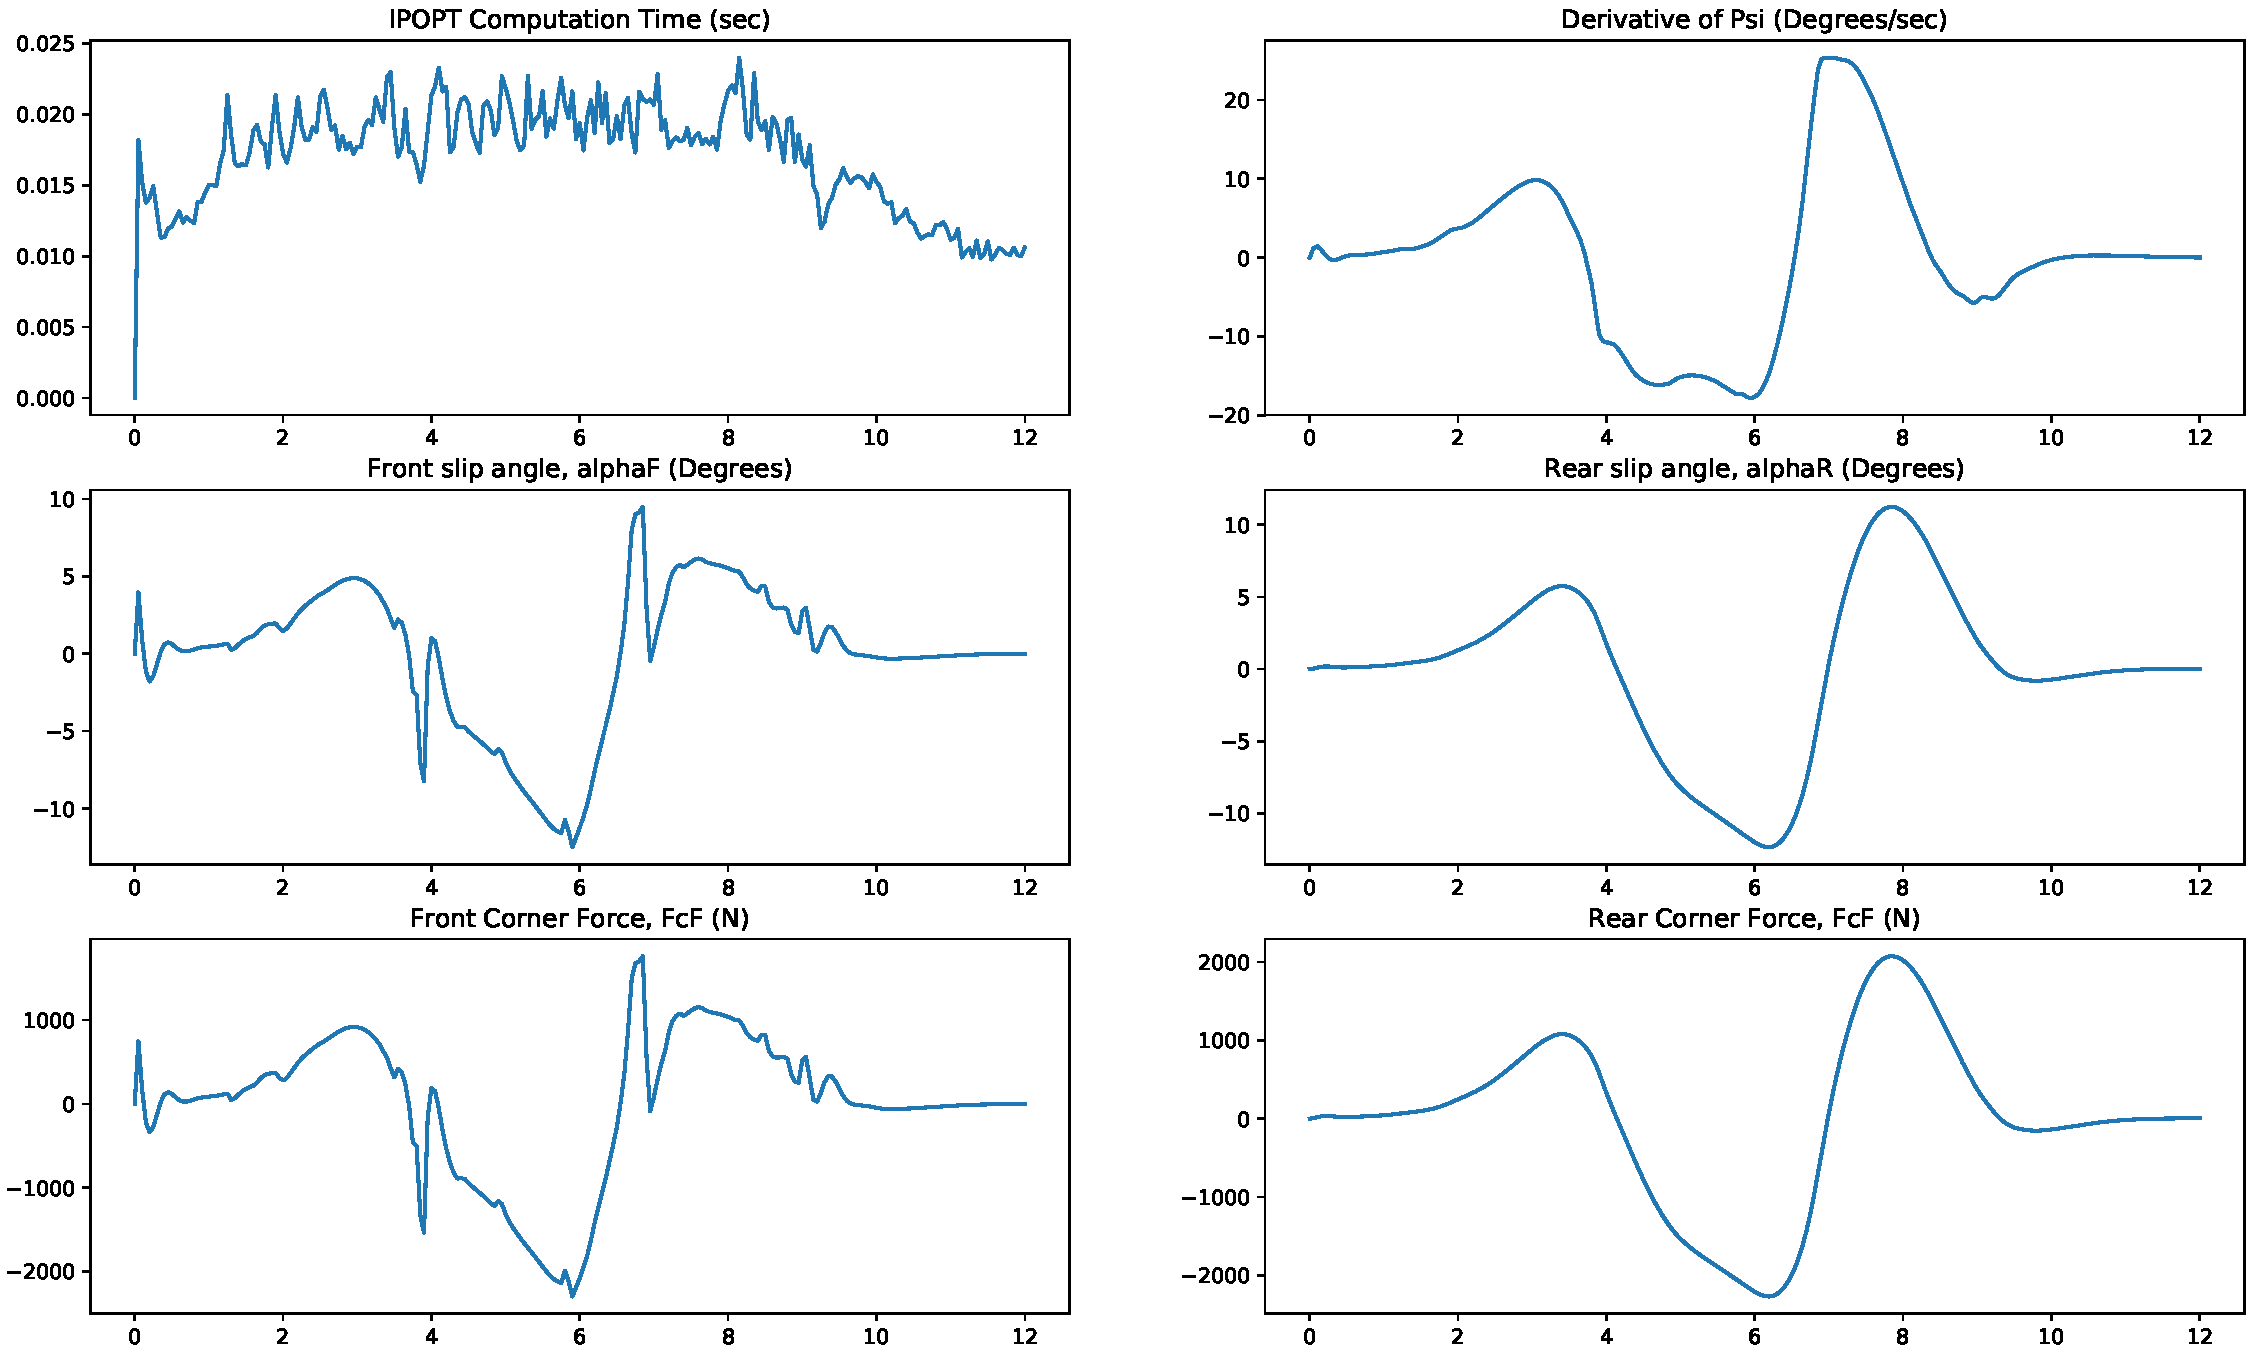
\includegraphics[width=0.95\textwidth,keepaspectratio]{images/Double_Lane_Change_Maneuver_cpp_02.pdf}
	\caption{(c++) Double lane change maneuver at $10$ m/s with $H_p$ $=$ $20$ and $H_c$ $=$ $20$. yaw rate, tire forces and slip angles.}
	\label{fig_11:double_lane_change_maneuver_02}
\end{figure}

\clearpage
\bibliography{references}
% You can use full name of authors, however most likely some of the Bibtex entries you will find, will use abbreviated first names
% If you don't want to correct each of them by hand, you can use abbreviated style for all of the references
\bibliographystyle{abbrv}
\clearpage

\end{document}